% Dokumentenklasse
\documentclass{article}

% deutsche Silbentrennung
\usepackage[ngerman]{babel}

% Tabellenpaket
\usepackage{tabularx}

% Umlaute
\usepackage[utf8]{inputenc}

% Fließobjekte
\usepackage{float}

% Mathepaket
\usepackage{amsmath}

% Bilder
\usepackage{graphicx}

% Für schräge Bruchstriche
\usepackage{nicefrac}

% Für Bilderformatierung
\usepackage{float}

% PDFs anhängen
\usepackage{pdfpages}

% Hyperref
\usepackage{hyperref}

% Literaturverzeichnis
\usepackage{cite}

% Latexbilder
\usepackage{tikz}

\bibliographystyle{unsrt} % <- Choose a style. Your document class may do this for you.
\bibliography{my-biblio}


\begin{document}

\begin{titlepage}
\centering
Protokoll zum Fortgeschrittenenpraktikumsversuch\\[2cm]\Huge
\vfill
\Huge
Zeitkorrelierte Einzelphotonenzählung\\[2cm]\Large
WS 2016/2017 \\
\vfill
\normalsize
\begin{tabular}{lcr}
Verfasser 1:   &   & Christoph Egerland       \\
Verfasser 2:   &   & Max Pfeifer              \\
Versuchsdatum: &   & 6.12.2016                \\
Versuchsplatz: &   & NEW15 2'106              \\
Betreuer:      &   & Dr. Steffen Hackbarth    \\
\end{tabular}
\end{titlepage}

\begin{center}
  \textbf{Abstract}
\end{center}
Mit Hilfe der zeitkorrelierten Einzelphotonenzählung (TCSPC) wird in diesem Versuch die Fluoreszenzlebensdauer von Phäophorbid a in Ethanol-Wasser-Gemischen untersucht.
Hierbei gehen wir insbesondere auf das Verhalten bei unterschiedlichen Konzentrationen, optischen Dichten und
zusätzlichen Reaktionsagenten (Triton X-100) der Probe ein. Es werden Störeffekte (Peak Pile-Up, Reabsorption) behandelt und quantifiziert.
Schließlich wird die Einbettung des Phäophorbid in Mizellen durch Messung der Anisotropie nachgewiesen.

\tableofcontents
\newpage


\section{Materialien und Methoden}
\subsection{Versuchsaufbau}
Der Versuchsaufbau wird in [1] beschrieben:\\
"Der Laser emittiert einen gepulsten Laserstrahl, der auf einen halbdurchlässigen Spiegel trifft.
Dieser teilt den Strahlenweg in zwei Komponenten. Der eine trifft auf eine Referenzdiode. Der
andere wird mit Hilfe eines $\lambda$/2-Plättchens und eines vertikal orientierten Polarisationsfilters
abgeschwächt und trifft anschließend auf die Probe. [...] Bei dem Detektor handelt es sich
um einen Photomultiplier dessen Pulse einen Constant Fraction Discriminator passieren
müssen, um gemessen zu werden."
\begin{figure}[h]
  \centering
  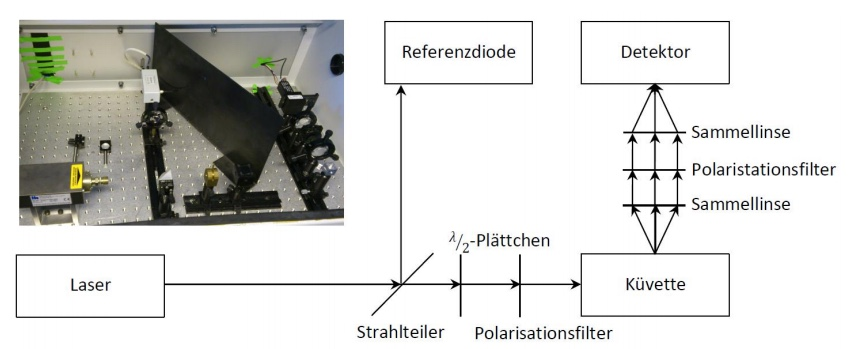
\includegraphics[width=\textwidth]{Bilder/aufbau.jpeg}
  \caption{Versuchsaufbau}
\end{figure}
\\
\\
Die Messelektronik stammt von der Firma Becker und Hickl GmbH, wir verwenden das Programm SPC300 dieser Firma.


\subsection{Versuchsmethode}
Die verwendete Versuchsmethode wird wie folgt in [1] beschrieben: \\
"Mit der TCSPC sollen strahlende optische Übergänge im Bereich vieler ps bis vieler ns
untersucht werden. Nun entsteht aber wegen der Unschärferelation im Allgemeinen das
Problem, nicht gleichzeitig schnell und genau messen zu können. Bei der TCSPC wird dieses
Problem durch die Entkopplung von Detektion und Zeitmessung umgangen. Die Grundidee ist
hierbei, dass sich eine Vielzahl identischer, nicht wechselwirkender Teilchen (oder Moleküle)
statistisch genauso verhält wie ein einzelnes Teilchen (oder Molekül)."

\section{Auswertung und Diskussion}
\subsection{Optimierung des Messplatzes}
In diesem Versuchsteil wollen wir eine optimale Konfiguration (optimal bedeutet hier: höchstmögliches
Signal-Rausch-Verhältnis SNR) erreichen. Wir setzen zunächst eine Streuküvette mit stark verdünntem
Ludox ein, stellen die Detektorspannung auf $U_D=800V$ und regeln die Laserintensität mit dem Polarisationsfilter so niedrig
wie möglich. In Tabelle 1 ist das SNR für die verschiedenen Schwellwerte des Constant-Fraction-Discriminators (CFD) dargestellt.
Wir erreichen das höchste SNR bei: $$CFD_{opt}=30mV$$

\begin{table}[h]
  \centering
  \begin{tabular}{c|c|c|c}
    CFD[mV] & Signal[Counts] & Rauschen[Counts] & SNR \\
    \hline
    5       &     -          & -                & -\\
    10      & 45000          & 200              & 225\\
    15      & 40000          & 50               & 800\\
    20      & 30000          & 10               & 3000\\
    25      & 25000          & 8                & 3125\\
    \textbf{30}      & \textbf{20000}          & \textbf{6}                & \textbf{3333.3}\\
    35      & 15000          & 5                & 3000\\
    40      & 12000          & 4                & 3000\\
    45      & 8000           & 3                & 2666.7\\
    50      & 5200           & 2                & 2600\\
  \end{tabular}
  \caption{Ermittlung des optimalen Schwellenwerts CFD bei $U=800V$}
\end{table}

Nun variieren wir mit festem Schwellwert $CFD_{opt}$ die Detektorspannung. In Tabelle 2 sehen wir analog zu
Tabelle 1 die Detektorspannung und das daraus resultierende SNR. Wir finden: $$ U_{opt}=800V$$


\begin{table}[h]
  \centering
  \begin{tabular}{c|c|c|c}
    U[kV] & Signal[Counts] & Rauschen[Counts] & SNR \\
    \hline
    0.6   &     0          & 0                & -\\
    0.7   &    520         & 2                & 260\\
    \textbf{0.8}   &  \textbf{16000}         & \textbf{5}                & \textbf{3200}\\
    0.9   &     25000      & 8                & 3125\\
    1.0   &     10000      & 5                & 2000\\
  \end{tabular}
  \caption{Ermittlung der optimalen Spannung bei $CFD_{opt}=30mV$}
\end{table}

In den folgenden Versuchsteilen werden wir also stets die feste Konfiguration $CFD_{opt}=30mV$ und $ U_{opt}=800V$ verwenden!

\subsubsection{Apparatefunktion}
Die aufgenommen Apparatefunktion der Streuküvette ist in Abbildung 2 dargestellt. Durch variieren der Countrate ergaben sich
kleine Variationen in der Halbwertsbreite des Peaks, sowie veränderte Fluktuationen in der auslaufenden Kurve. Es wurde jene Countrate
gewählt, bei der eine weitere Verringung die Halbwertsbreite nicht weiter verringert. Am Graphen ist diese gut zu sehen:
$$Countrate \approx \mathcal{O}(10^4)$$

\begin{figure}[h]
  \centering
  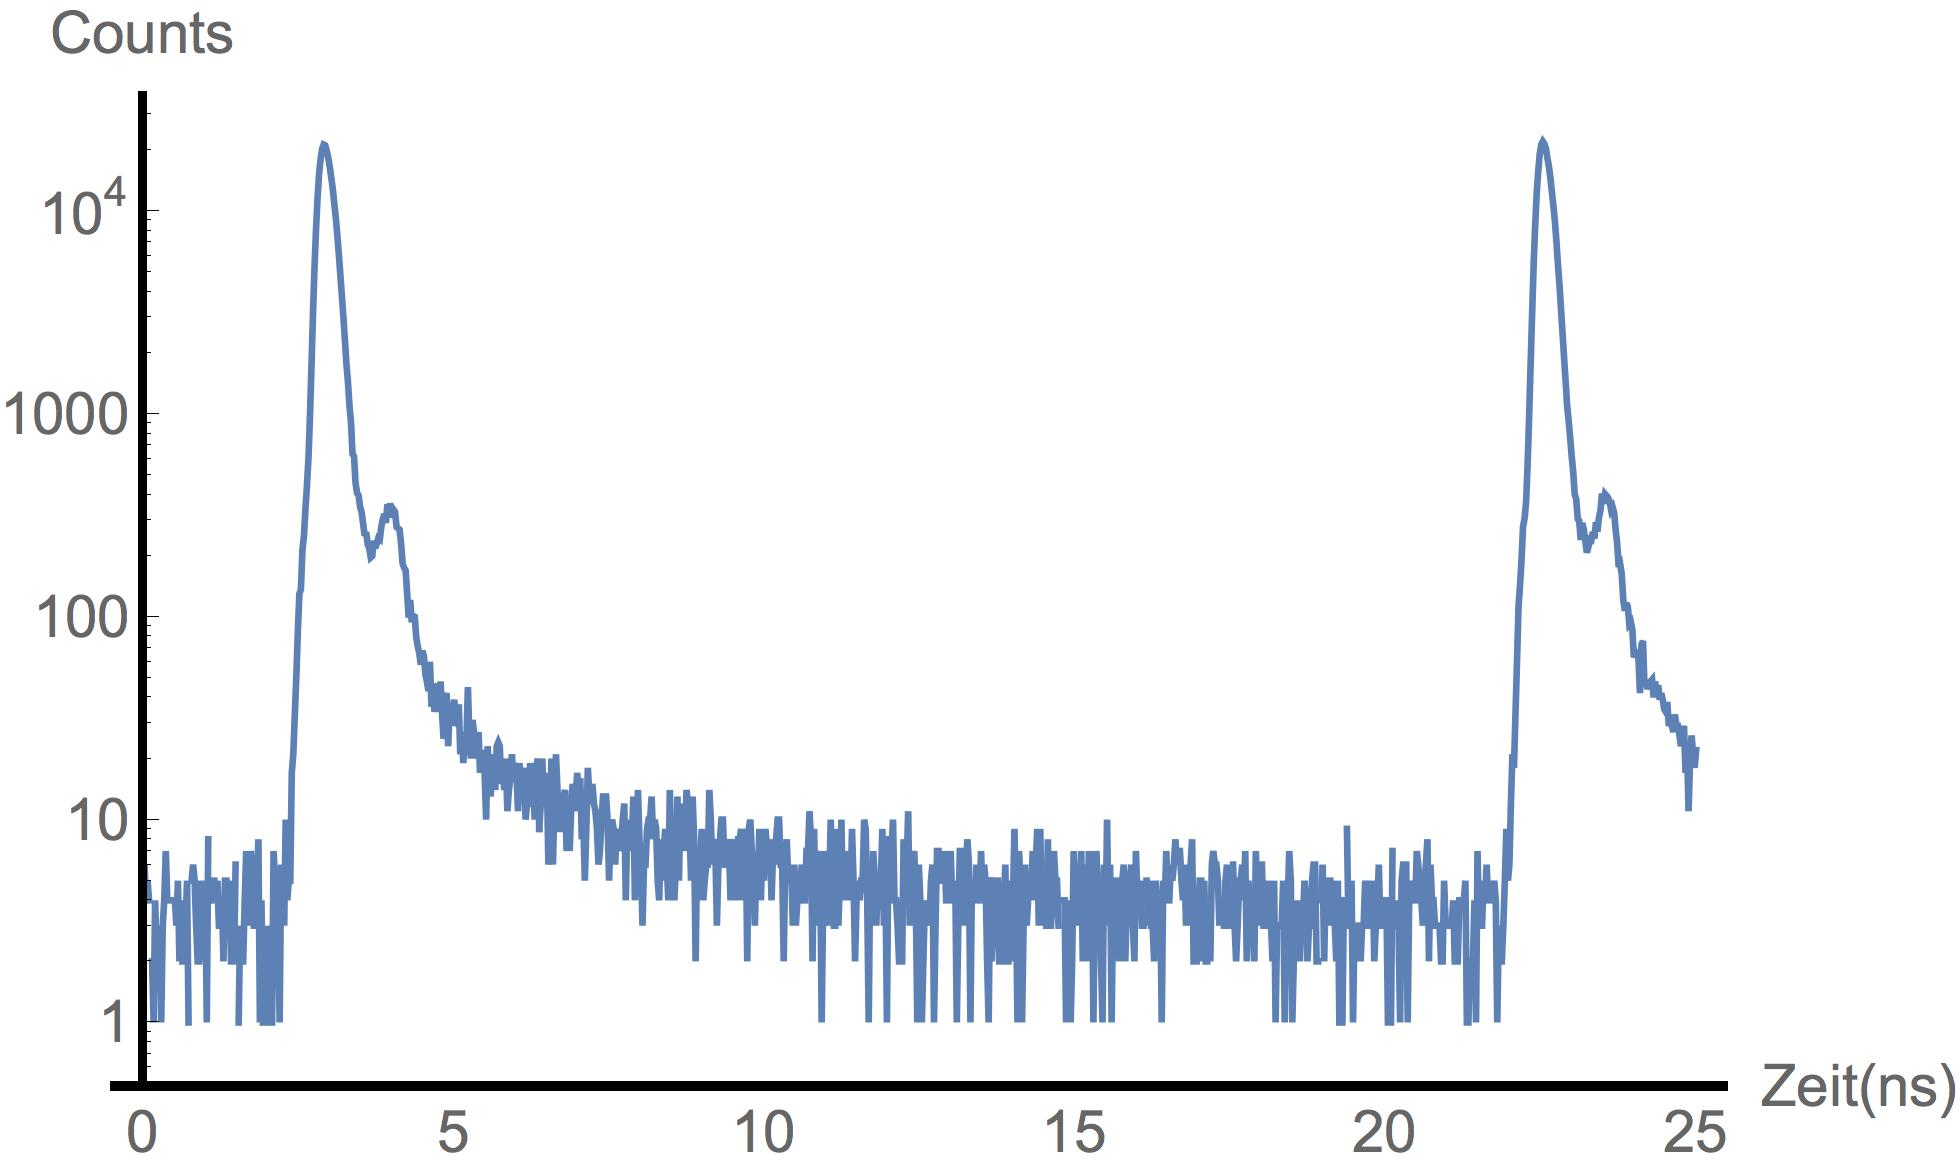
\includegraphics[width=\textwidth]{Bilder/apparatekurve.jpg}
  \caption{Apparatekurve}
\end{figure}



\subsubsection{Peak-Pile-Up-Effekt}
Unter dem Peak-Pile-Up-Effekt versteht man, dass zwei Photonen nicht als zwei separate Events registriert werden. Wir erwarten,
dass bei höherer Laserintensität zum einen die Amplitude $A$ größer wird und dass die Fluoreszenzlebensdauer $t$ abnimmt, da es bei
höheren Intensitäten wahrscheinlicher ist, dass zwei Photonen als ein Ereignis gezählt werden und somit nicht doppelt zur Kurve beitragen.
Die Messung wurde mit einer Probe mit $OD = 0.1$ und verschiedenen Laserintensitäten durchgeführt.

\begin{table}[h]
  \centering
  \begin{tabular}{c|c|c|c}
    I[$\mu$W]      & A[a.u.]  & t[ns]             & $\chi^2$\\
    \hline
    15.9            &  0.19    & 5.44              & 1.42    \\
    77              &  0.19    & 5.42              & 1.42    \\
    79              &  1.06    & 5.38              & 2.06    \\
    91              &  1.24    & 5.44              & 2.24    \\
  \end{tabular}
  \caption{Messung des Peak-Pile-Up-Effekts}
\end{table}


Die Ergebnisse der Messung sind in Tabelle 3 aufgeführt. Die Fits zeigen eine gute Übereinstimmung zum Modell ($\chi^2-Werte < 2.3$)
und die oben beschriebenen Erwartungen werden bestätigt. Die Halbwertszeit nimmt mit zunehmender Intensität ab, die Amplitude steigt.
Allerdings liegt die Schwankung lediglich in der Fehlerordnung und ist somit also zu vernachlässigen. Wir wählen $I = 77 \mu W$ als
Laserintensität für die folgenden Versuche.



\subsubsection{Reabsorption}
Für diesen Versuchsteil mussten zunächst 5 Proben mit verschiedener optischer Dichte im Bereich
$0.1$ - $1.5$ hergestellt werden. Hierfür wurde auf der Grundlage, dass die optische Dichte eines Stoffes
proportional zur Konzentration desselben ist, folgende Formel hergeleitet:

\begin{equation}
  \omega = \frac{V_{Pheo}}{V_{Rest}}=\frac{OD_{Probe}}{OD_{Pheo}-OD_{Probe}}
\end{equation}



Hierbei ist $OD_x$ die optische Dichte des jeweiligen Stoffes. Für ein Probenvolumen von $2ml$ und eine
optische Dichte des Pheophorbid a von $OD_{Pheo}=2.4$ ergeben sich die Werte wie in Tabelle ZAHL.

\begin{table}[h]
  \centering
  \begin{tabular}{c|c|c|c}
    $OD_{Probe}$ & $\omega$ & $V_{Pheo}$[$\mu$l] & $V_{Ethanol}$[$\mu$l] \\
    \hline
    0.1          &  1:23  & 87                & 1913 \\
    0.3          &  1:7   & 250               & 1750 \\
    0.7          &  7:17  & 583               & 1417 \\
    1.1          &  11:13 & 917               & 1083 \\
    1.5          &  5:3   & 1250              & 750  \\
  \end{tabular}
  \caption{Mischung der Proben für verschiedene optische Dichten}
\end{table}



Unter Reabsorption versteht man, dass ein absorbiertes und wieder abgestrahltes Photon erneut absorbiert und emmitiert wird.
Wir erwarten also, da bei höheren optischer Dichte die Wahrscheinlichkeit für einen solchen Fall höher ist, dass die Fluoreszenzlebensdauer
bei höheren optischer Dichte steigt, da nun ein Photon zwei Counts verursacht. Die Ergebnisse der Messung befinden sich in Tabelle 5.


\begin{table}[h]
  \centering
  \begin{tabular}{c|c|c|c}
    OD           & A[a.u.]& t[ns]             & $\chi^2$\\
    \hline
    0.2          &  0.01  & 5.91              & 1.21  \\
    0.3          &  0.54  & 5.44              & 1.66  \\
    0.7          &  0.59  & 5.54              & 1.64  \\
    1.1          &  0.63  & 5.62              & 1.79  \\
    1.5          &  0.27  & 5.86              & 1.50   \\
  \end{tabular}
  \caption{Messung Reabsorptionseffekt}
\end{table}


Die Fits zeigen wieder gute Übereinstimmung mit dem Modell ($\chi^2-Werte <2$) und unsere Erwartungen bestätigen sich deutlich.
Die Fluoreszenzlebensdauer steigt bei höheren Dichte um bis zu 8\% an. Im Folgenden werden wir also $OD = 0.2$ wählen.




\subsection{Fluoreszenzlebensdauer von Pheo}
Nun wird die Fluoreszenzlebensdauer bei den optimalen Einstellung bestimmt. Diese sind noch einmal zusammengefasst:

\begin{itemize}
  \item CFD-Spannung: $CFD_{opt}=30mV$
  \item Detektorspannung: $U_D=800V$
  \item Laserintensität: $I=77\mu W$
  \item optische Dichte der Probe: $OD=0.2$
\end{itemize}

Die Fluoreszenzlebensdauer ist: $$t=(5.9 \pm 0.1)ns$$
Diese stimmt sehr gut mit dem Referenzwert in [2] überein (ebenfalls $t=(5.9 \pm 0.1)ns$). Auch der $\chi^2$-Wert weißt auf
eine sehr gute Übereinstimmung mit dem Modell hin.



\subsection{Pheo in versch. Ethanol-Wasser-Gemischen}
Für diesen Versuchsteil stellen wir 7 Proben mit verschiedenem Ethanol-Wasser-Verhältnis her.
Wir setzen in unserer $2ml$ Probe $V_{Pheo}=1ml$, so dass $V_{Rest}=1ml$. Mit $\omega= \frac{V_{Ethanol}}{V_{Rest}}$ erhalten wir:

\begin{table}[h]
  \centering
  \begin{tabular}{c|c|c}
    $\omega$ & $V_{H_2O}$ [$\mu$l] & $V_{Ethanol}$ [$\mu$l] \\
    \hline
     5\%     & 950                 & 50                     \\
     15\%    & 850                 & 150                    \\
     30\%    & 700                 & 300                    \\
     45\%    & 550                 & 450                    \\
     60\%    & 400                 & 600                    \\
     75\%    & 250                 & 750                    \\
     100\%   & 0                   & 1000                   \\

  \end{tabular}
  \caption{Mischung für verschiedene Verhältnisse Ethanol:Wasser}
\end{table}

Wir erwarten, dass bei höherem Anteil die Fluoreszenzlebensdauer sinkt, da Phäophorbid a schlecht wasserlöslich ist, im wässrigen Milieu also zur
Aggregation neigt.

\begin{figure}[h]
  \centering
  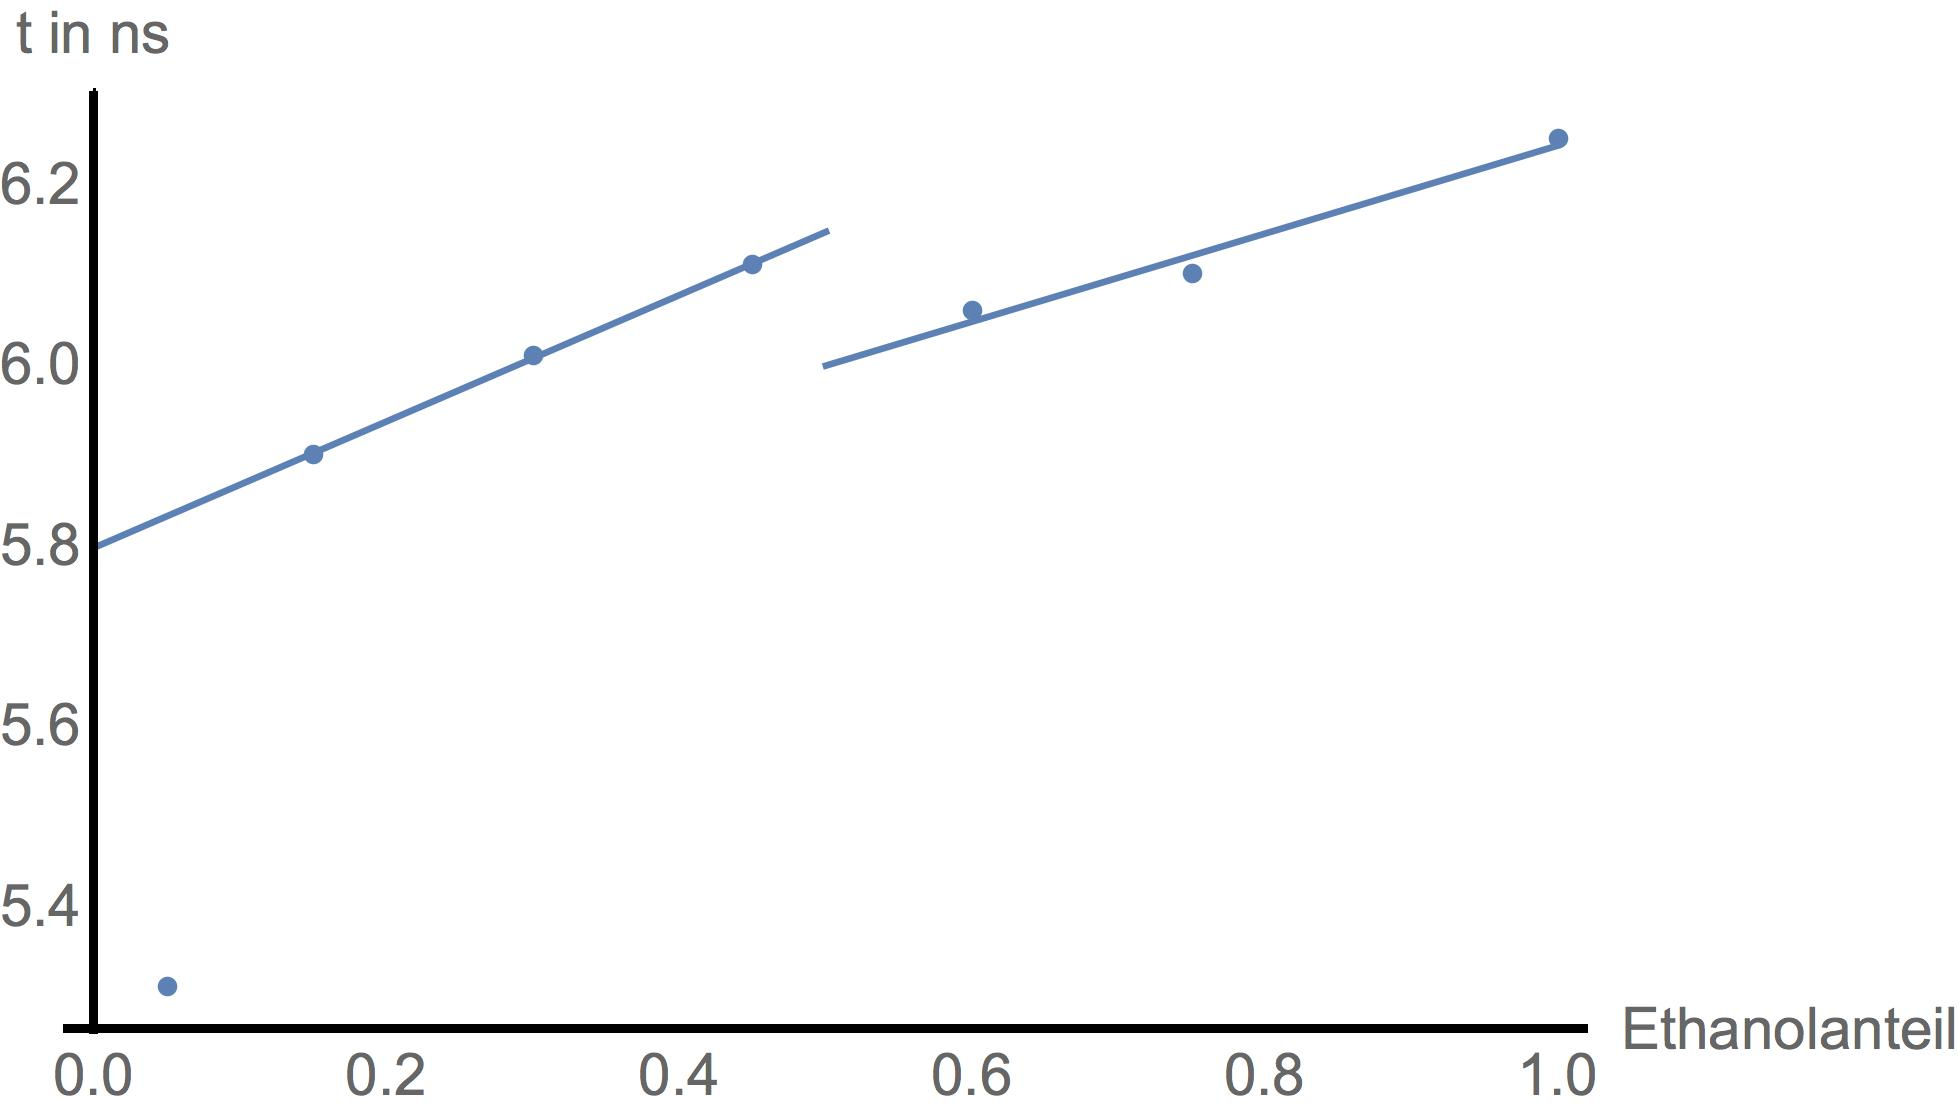
\includegraphics[width=\textwidth]{Bilder/FitEthH2O.jpg}
  \caption{Messung der Fluoreszenzlebensdauer für verschiedene Ethanol-Wasser-Verhältnisse}
\end{figure}

Die Ergebnisse sind in Abbildung 3 veranschaulicht. Man erkennt, dass die Fluoreszenzdauer sinkt, je höhere der Anteil von Wasser bzw.
umso niedriger der Anteil von Ethanol ist. Hierbei fällt die Fluoreszenzdauer bei Wasseranteilen $>50\%$ stärker ab, als bei Anteilen $<50\%$.
Der erste Messpunkt wurde bei der Regression nicht einbezogen, seine Lage legt nahe, dass es sich um eine Fehlmessung handelt. Eine schlechte Entscheidung
der Messenden war es eine Probe mit $OD = 1.5$ für die Messung zu verwenden, wo doch in Abschnitt 2.1.3 festgestellt wurde, dass hier der
Reabsorptionseffekt eine wesentliche Rolle spielt.






\subsection{Einbettung in Mizellen / Triton X-100}


\subsubsection{Wirkungsweise von Triton X-100}
"Triton X-100 ist ein Detergenz, welches Pheophorbid in Mizellen einbettet und so wasserlöslich
macht." ([1]) Wir geben nun zu der Probe mit höchstem Wasseranteil 2 Tropfen einer $10\%$igen Stammlösung Triton X-100
hinzu und erwarten, dass hierdurch die Fluoreszenzdauer wieder auf das optimale Niveau wie in Abschnitt 2.2 ansteigt.


\begin{figure}[h]
  \centering
  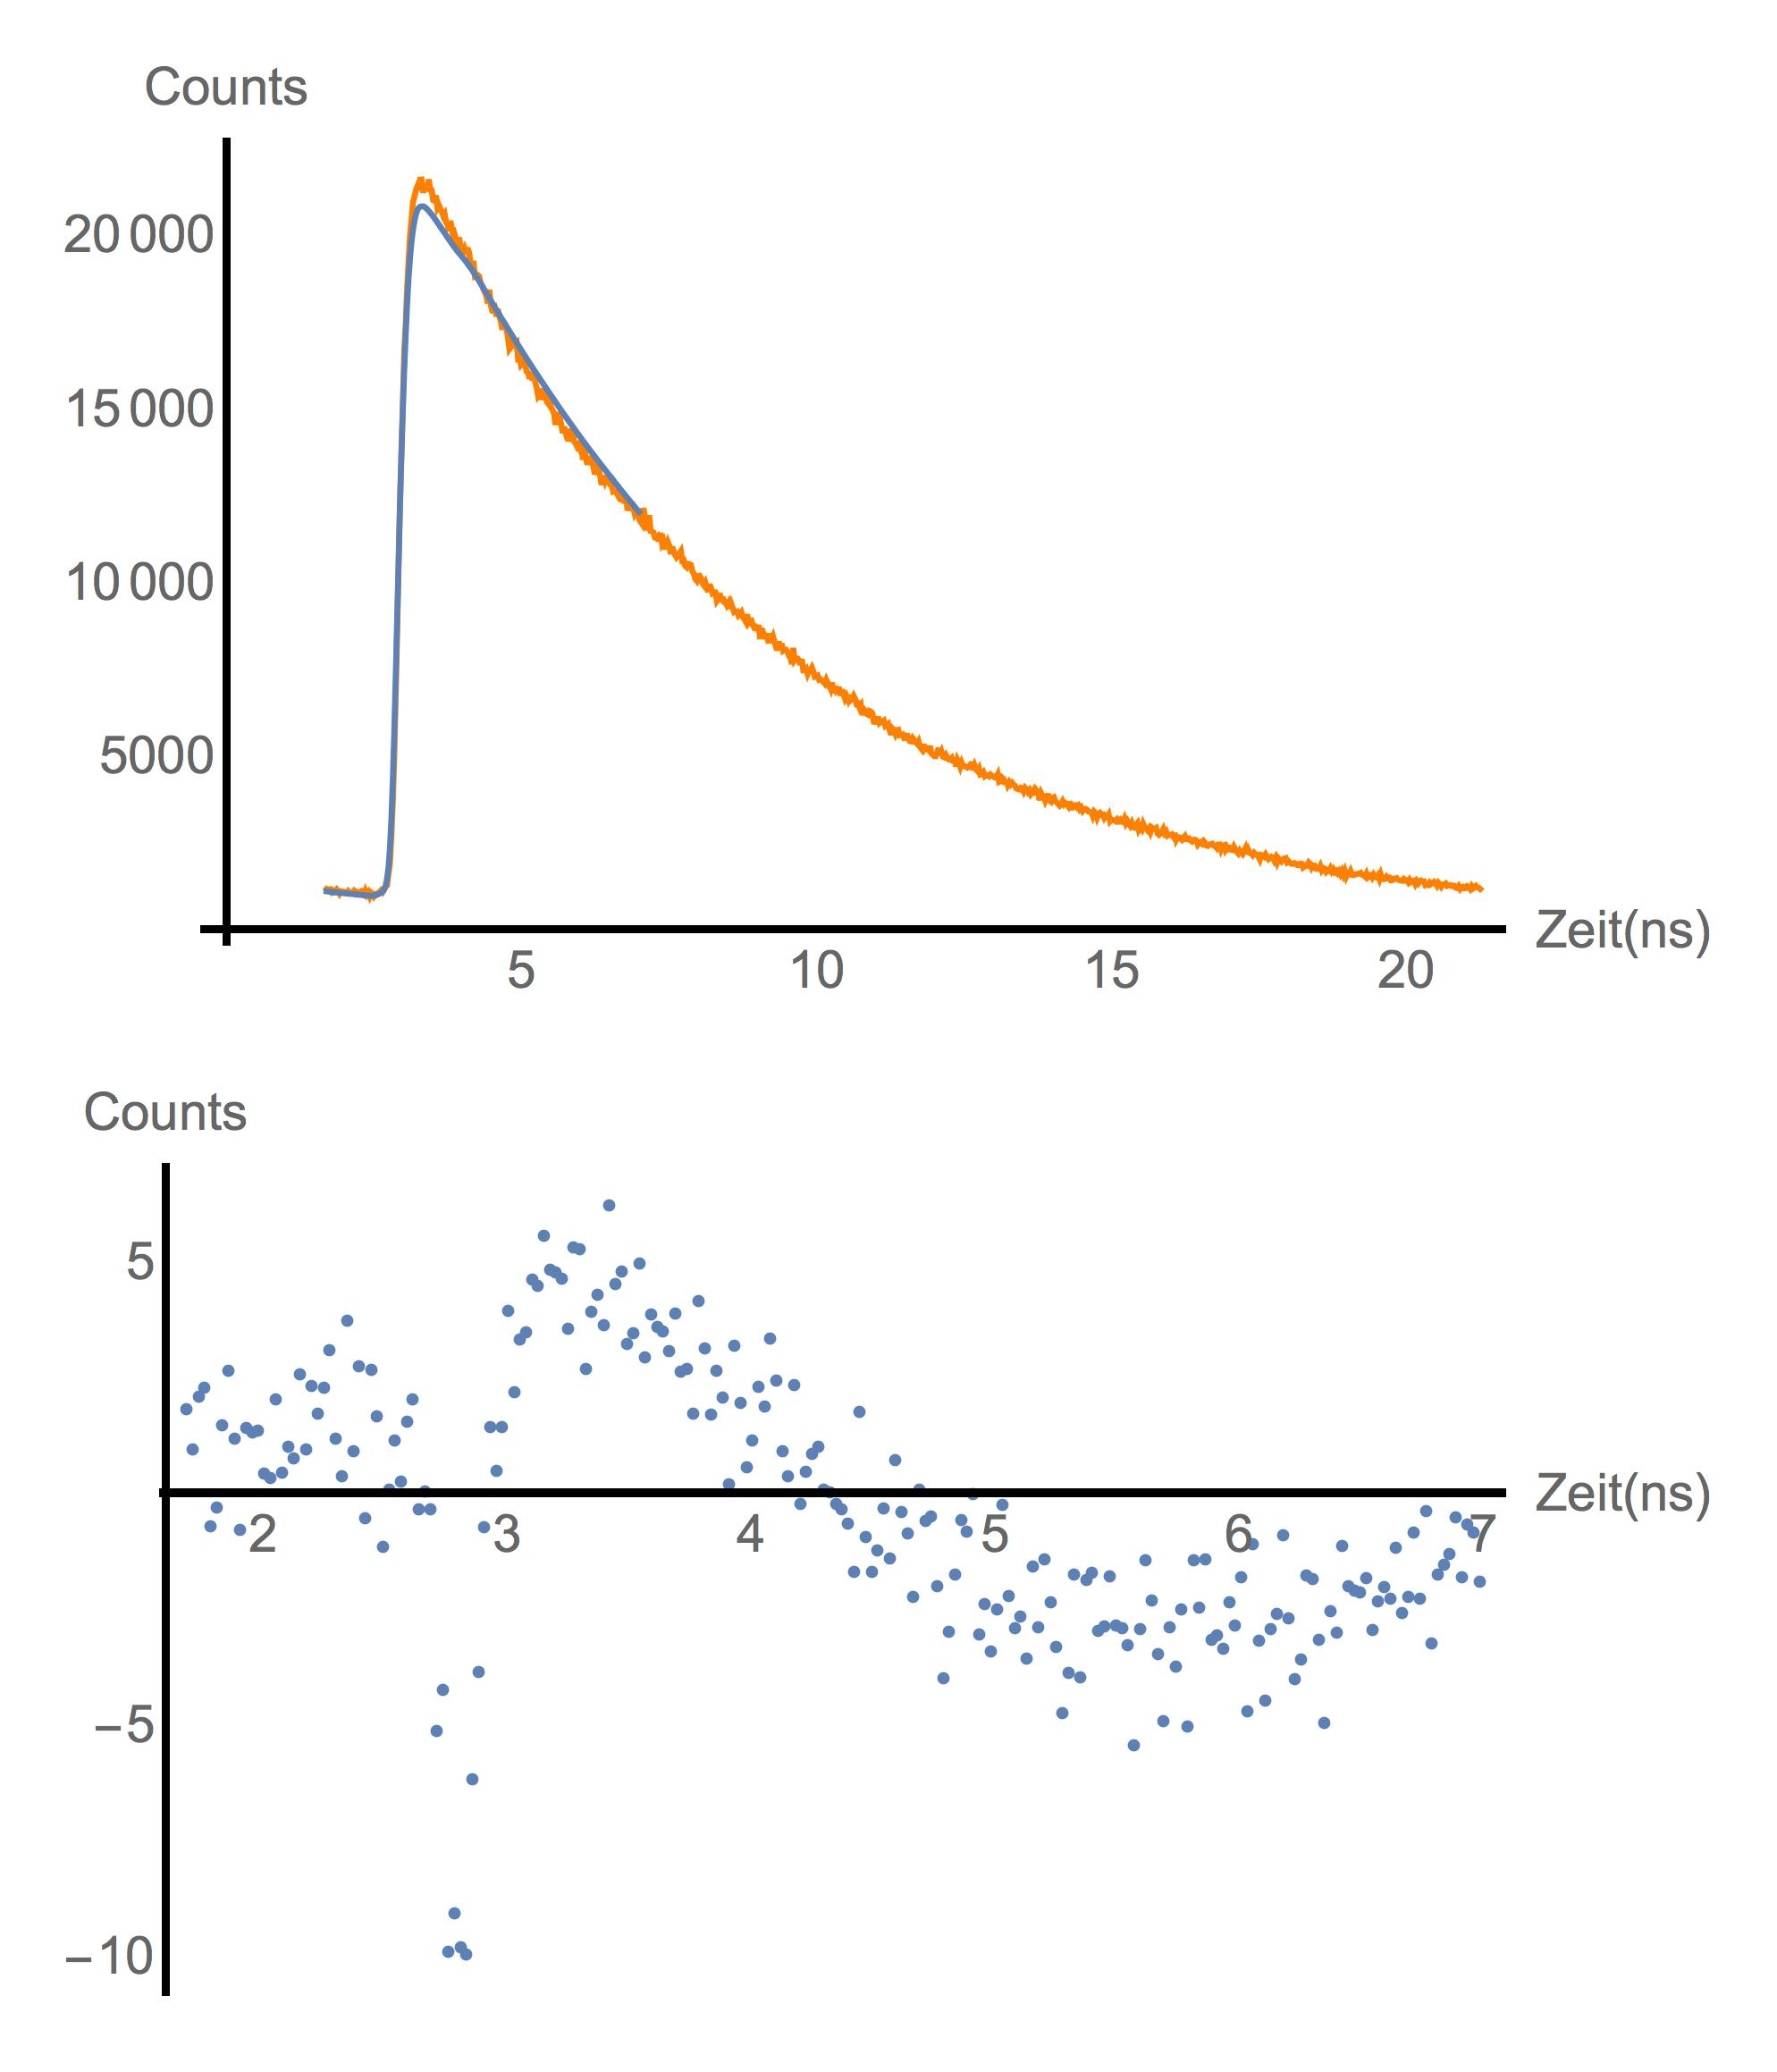
\includegraphics[width=\textwidth/2]{Bilder/FitTriton.jpg}
  \caption{Messung der Fluoreszenzlebensdauer mit Triton X-100, $t = 5.97ns$, $A = 0.26[a.u.]$, $\chi^2 = 2.94$}
\end{figure}

Die Fluoreszenzlebensdauer ist, wie nach Erwartung angestiegen, allerdings über die Fluoreszenzdauer in 2.2 hinaus. Dies liegt daran, dass
die Probe eine optische Dichte von $OD = 1.5$, der Reabsorptionseffekt trägt hier, wie in Abschnitt ZAHL gezeigt, eine tragende Rolle. Dies war
eine für präzise Messergebnisse ungünstige Wahl der Experimentatoren. Ebenso schlägt sich dies in einem (im Vergleich zu allen anderen Fits)
schlechten Chi2-Wert von $\chi^2=2.94$ nieder. Nichtsdestotrotz zeigt die Messung, dass Phäophorbid a durch das Triton X-100 wieder fluoresziert.


\begin{figure}[h]
  \centering
  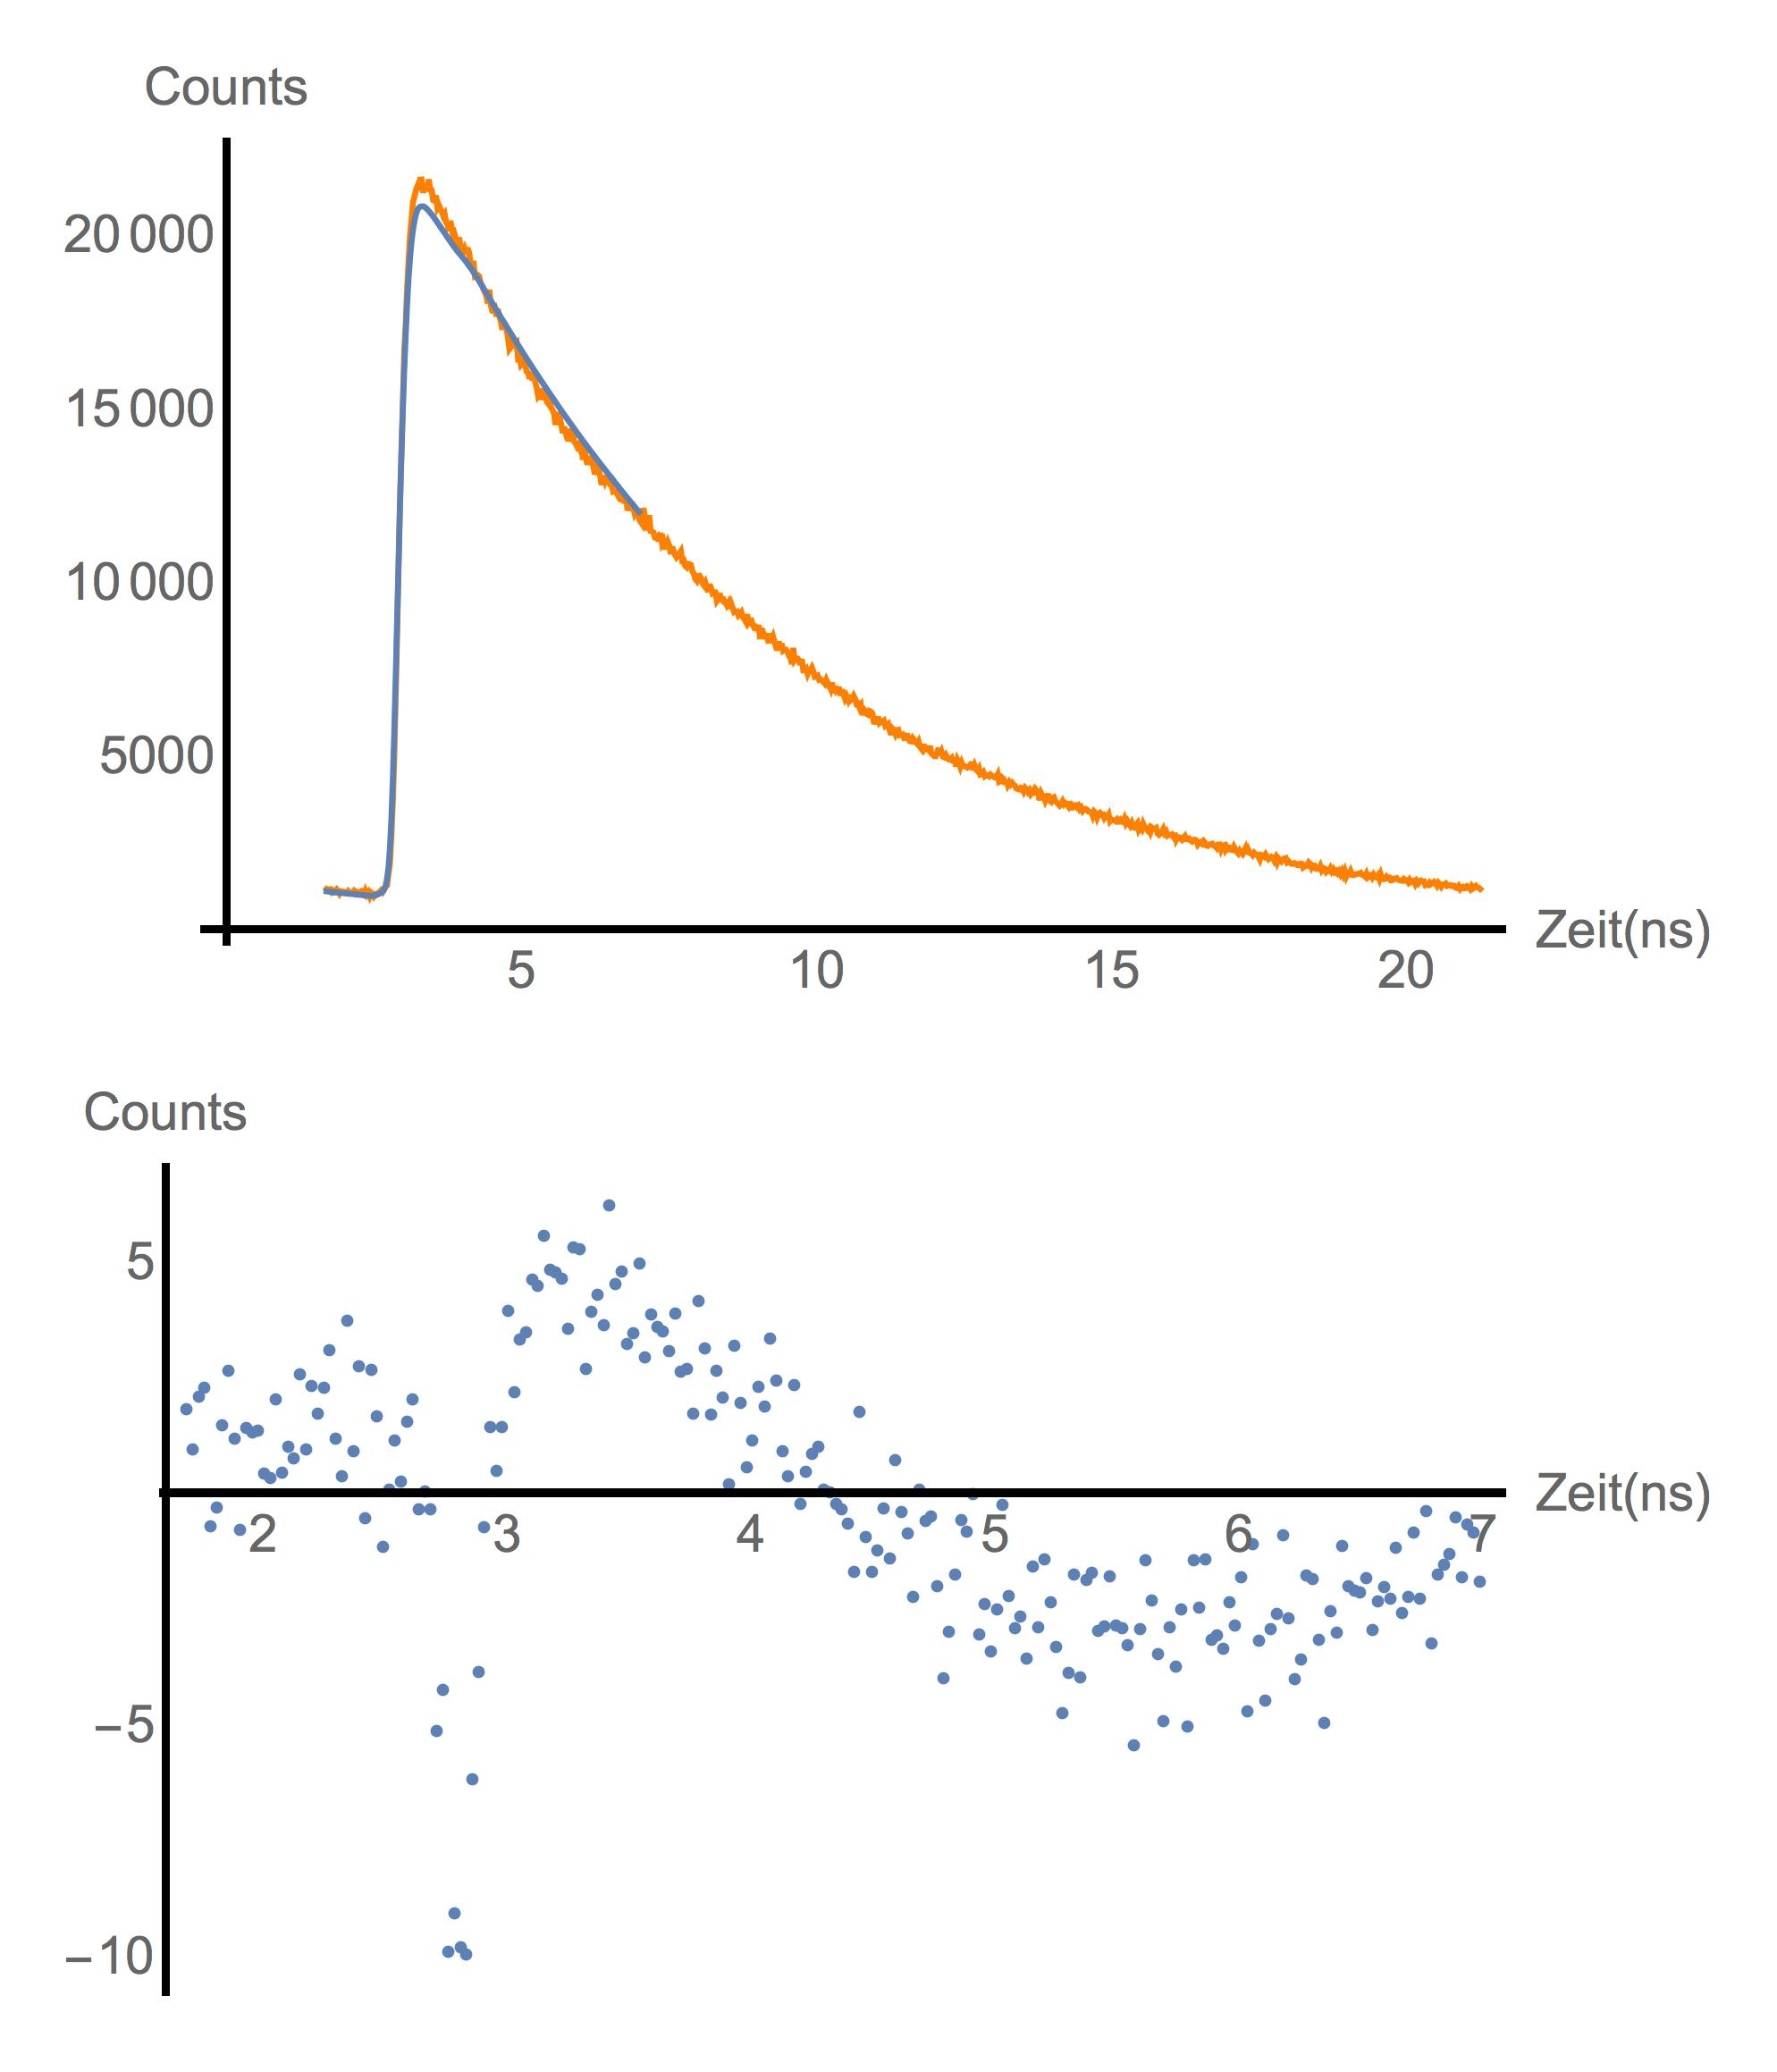
\includegraphics[width=\textwidth/2]{Bilder/FitTriton.jpg}
  \caption{Messung der Fluoreszenzlebensdauer mit Triton X-100, $t = 5.97ns$, $A = 0.26[a.u.]$, $\chi^2 = 2.94$}
\end{figure}

Die Fluoreszenzlebensdauer ist, wie nach Erwartung angestiegen, allerdings über die Fluoreszenzdauer in 2.2 hinaus. Dies liegt daran, dass
die Probe eine optische Dichte von $OD = 1.5$, der Reabsorptionseffekt trägt hier, wie in Abschnitt 2.1.3 gezeigt, eine tragende Rolle. Dies war
eine für präzise Messergebnisse ungünstige Wahl der Experimentatoren. Ebenso schlägt sich dies in einem (im Vergleich zu allen anderen Fits)
schlechten Chi2-Wert von $\chi^2=2.94$ nieder. Nichtsdestotrotz zeigt die Messung, dass Phäophorbid a durch das Triton X-100 wieder fluoresziert.




\subsubsection{Anisotropie}
Werden Fluorophore mit linear polarisiertem Licht bestrahlt absorbieren bevorzugt Moleküle, bei denen der Winkel zwischen Übergangsdipolmoment und Polarisationsebene des einfallenden Lichts klein ist. Dies führt i.A. dazu, dass das durch Fluoreszenz emittiertes Licht ebenso linear polarisiert ist - die sog. Fluoreszenzpolarisation. Diese intrinsische Anisotropie ist als Maß für den Grad der Polarisation des Emissionslichts abhängig von den Intensitäten des parallel bzw. senkrecht polarisierten Fluoreszenzlichts. $$ r = \frac{I_\parallel-I_\perp}{I_\parallel+2 I_\perp} $$ Zur quantitativen Bestimmung werden jene Polarisationsintensitäten bei fester (linearer) Polarisation des einfallenden Lichts gemessen. Die sog. Rotationsabklingzeit $\tau_{Rot}$ bestimmt gemäß eines exponentiellen Abfalls maßgeblich den zeitlichen Abfall der Anisotropie. Sie ist, neben der Viskosität und Temperatur, v.a. von der Molekülgröße (Volumen) abhängig. Es wurden zwei Proben untersucht: Pheo in Ethanol und Pheo in einem Wasser/Triton-Gemisch.

\begin{figure}[H]
  \centering
  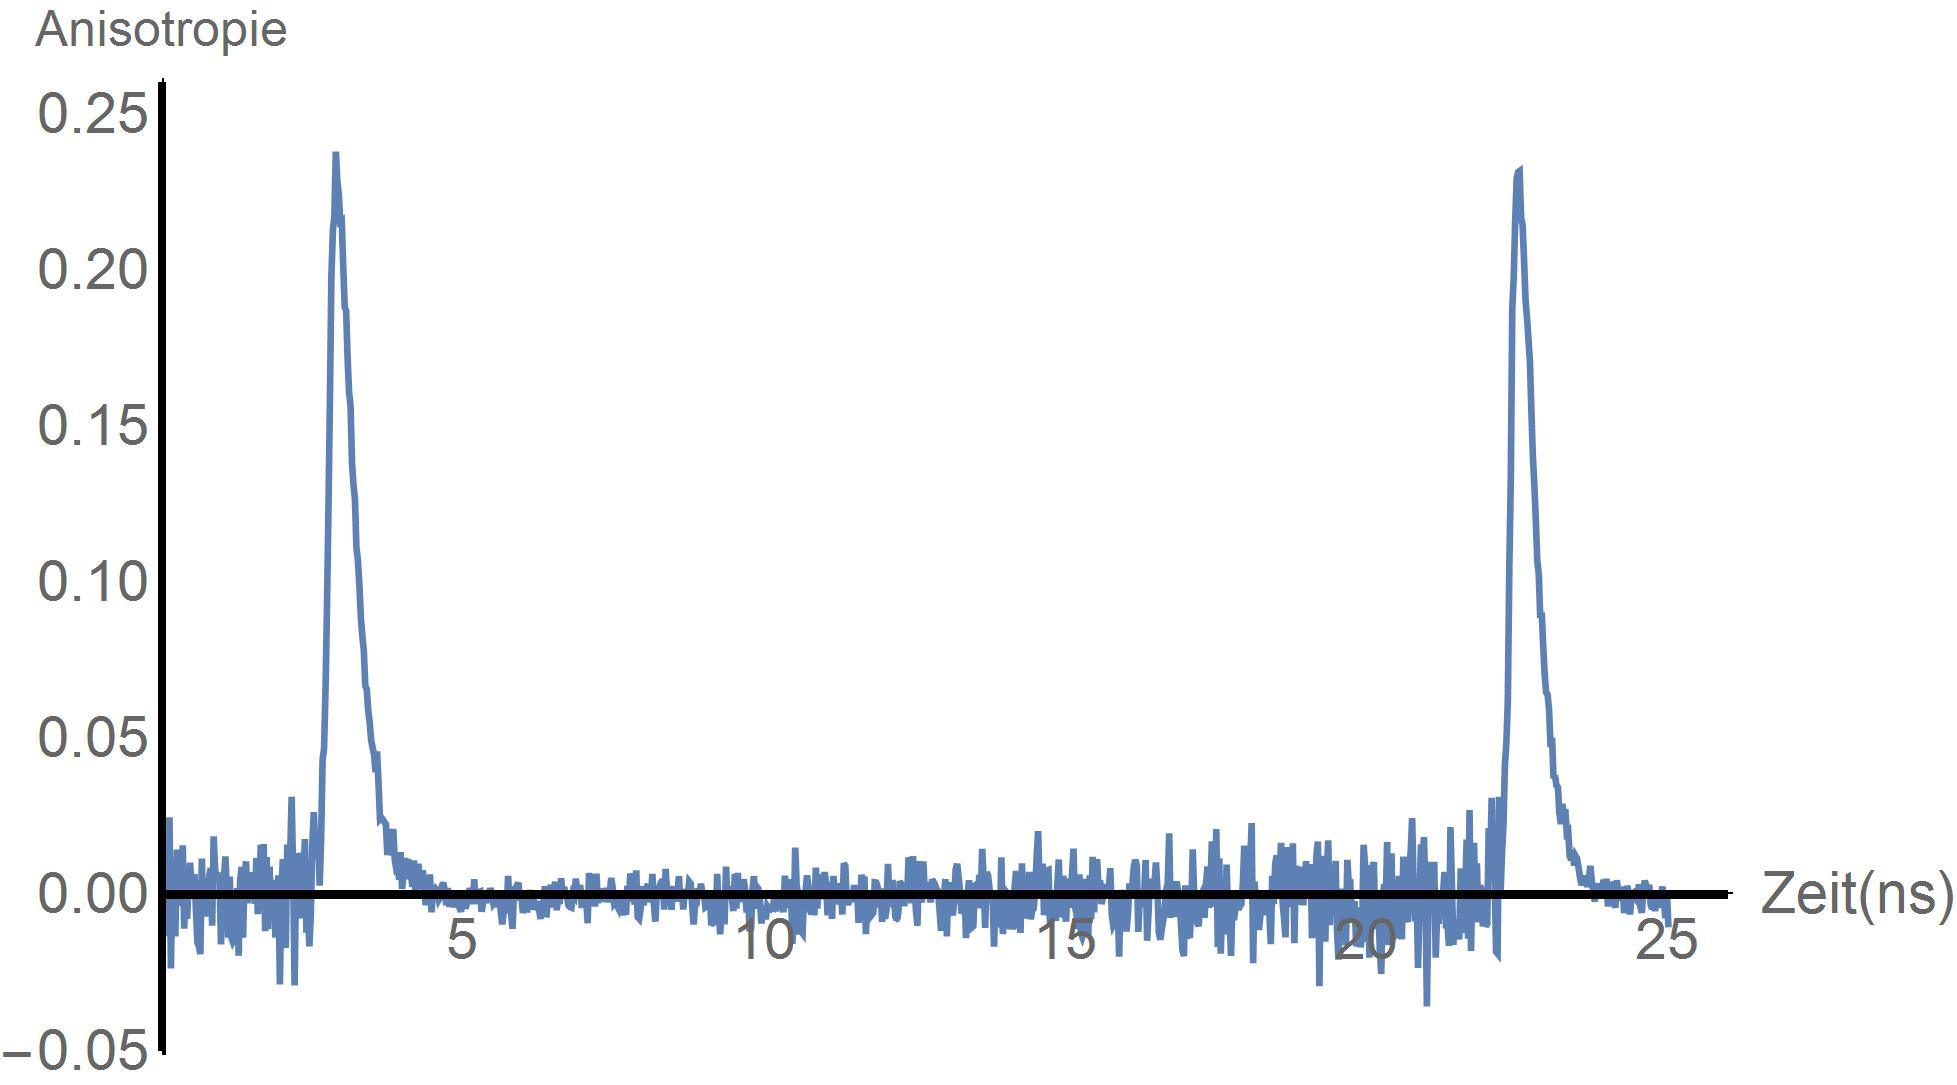
\includegraphics[width=\textwidth]{Bilder/anisotropie_ethanol.jpg}
  \caption{Messung der Anisotropie von Phäophorbid a mit Ethanol}
\end{figure}

Deutlich zu erkennen auf den Abb. 6 und 7 sind die beiden Anisotropie-Peaks bei den Fluoreszenzereignissen und der exponentielle Charakter des Abklingens der Anisotropie.

\begin{figure}[H]
  \centering
  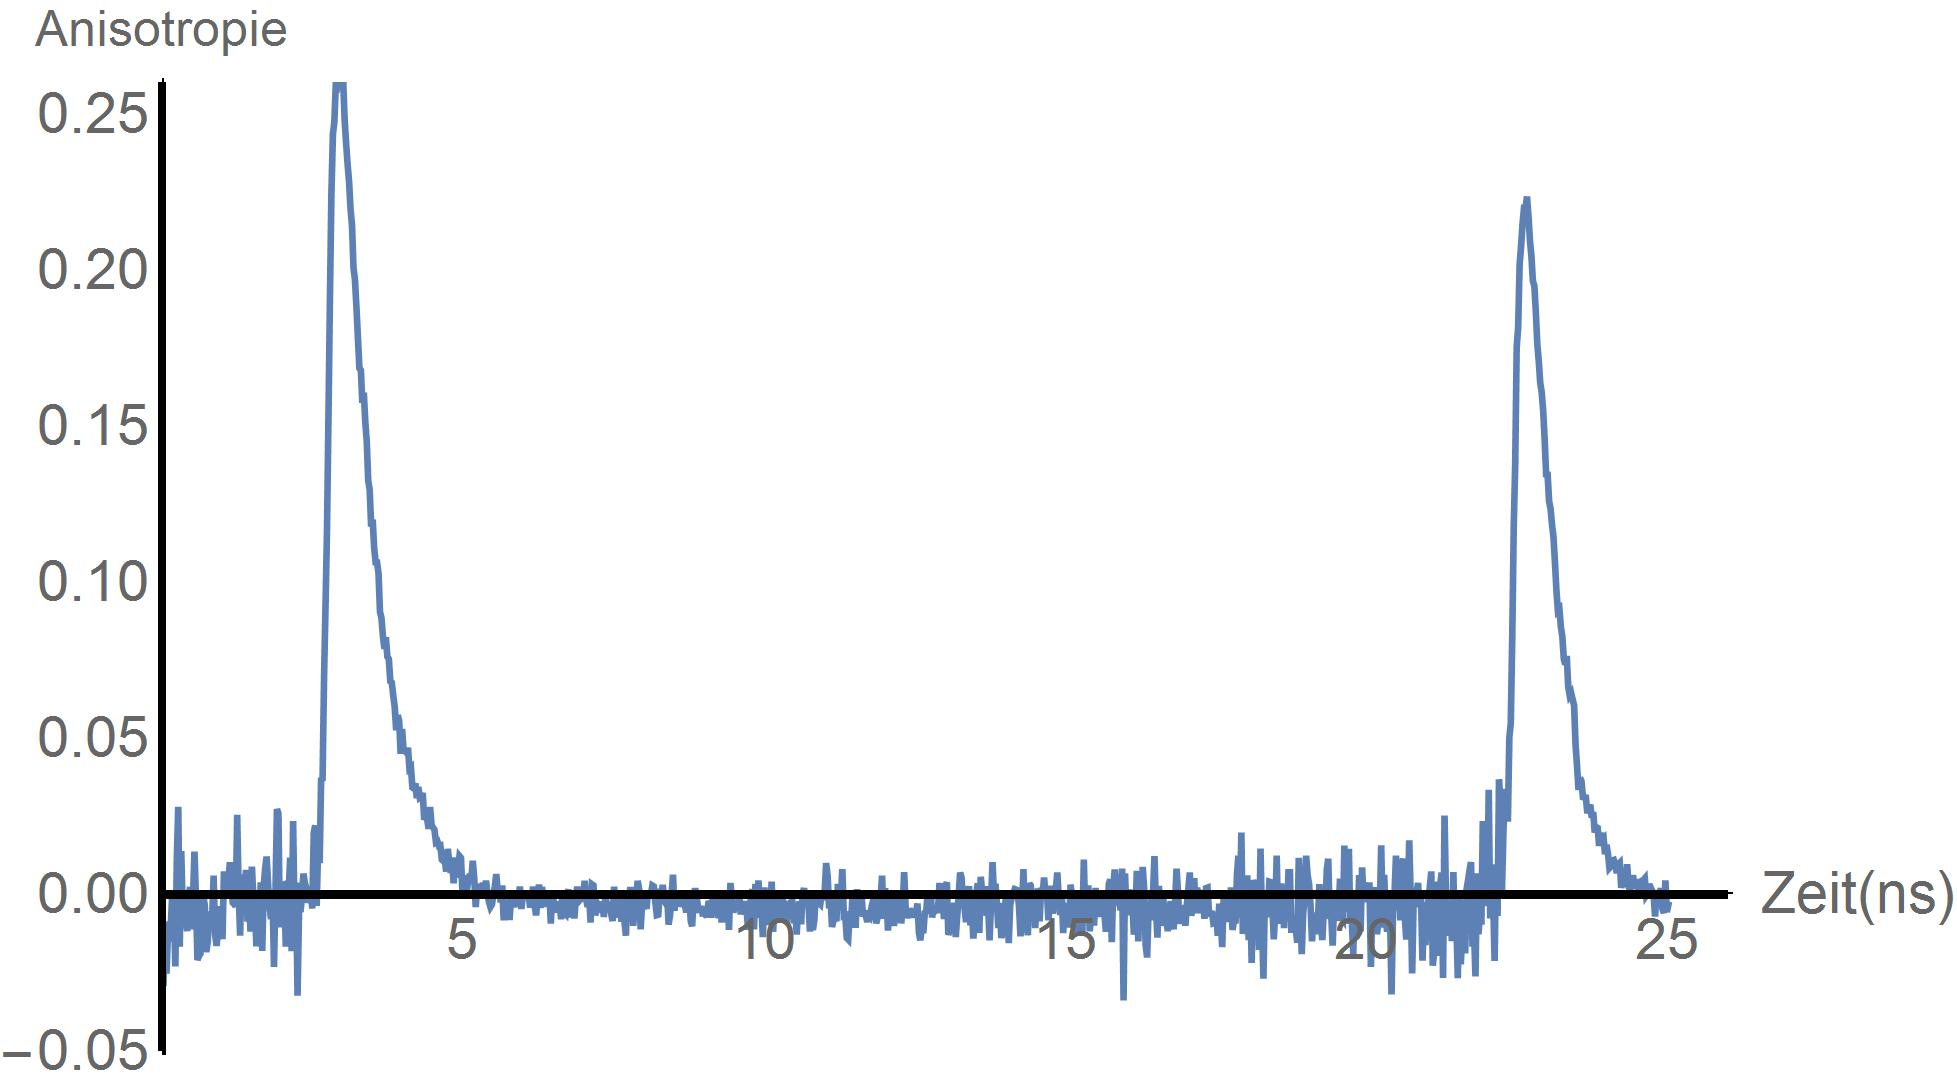
\includegraphics[width=\textwidth]{Bilder/anisotropie_triton.jpg}
  \caption{Messung der Anisotropie von Phäophorbid a mit einem Triton/Wasser-Gemisch}
\end{figure}


\newpage

Den Erwartungen entsprechend ist die Abklingzeit der Anisotropie bei der Probe mit Ethanol (Abb. 5) kürzer als bei jener mit dem Triton/Wasser-Gemisch (Abb. 6). Die Rotationsabklingzeit $\tau_{Rot}$ nimmt gemäß $$ \tau_{Rot}=\frac{\eta V}{k_B T} $$
mit größerem Volumen zu, wohingegen die Anisotropieabklingzeit nach $$ r= c \cdot e^{-\nicefrac{t}{\tau_{Rot}}}+d $$
invers proportional zur Rotationsabklingzeit ist. Das kürzere Abklingen der Anisotropie von Pheo in Wasser/Triton als in Ethanol spricht also für eine längere Rotationsabklingzeit und damit für ein größeres Volumen der fluoreszierenden Moleküle. Dies weist deutlich auf die erwartete Einbettung von Pheo in Mizellen im Wasser/Triton-Gemisch hin.



\section{Schlussfolgerungen}
Der ermittelte Basiswert für die Fluoreszenzlebensdauer von $t=(5.9 \pm 0.1)$ ns deckt sich genau mit dem Referenzwert aus [2] (S. 41, Tabelle).

Die auftretenden Störeffekte (Peak-Pile-Up, Reabsorption) konnten qualitativ nachgewiesen werden.


Die im Rahmen der Untersuchungen zur Löslichkeit von Phäophorbid a in Wasser/Ethanol-Gemischen ermittelten Fluoreszenzlebensdauern (Abs. 2.3) zeigen deutlich die hydrophobe Eigenschaft des Fluorophors. Dabei hätte man bei der Probe mit maximalem Wasseranteil keine Fluoreszenz bzw. zumindest eine deutlich niedrigere Fluoreszenzlebensdauer erwartet. Jedoch verschwindet die Fluoreszenzlebensdauer aufgrund der ungünstigen Wahl der Volumenaufteilung in der Probe (1 ml Phäophorbid a, 1 ml Wasser/Ethanol) nicht.

Die Zugabe von Triton X-100 zur Probe mit maximalem Wasseranteil lässt die Fluoreszenzlebensdauer ansteigen und entspricht damit den theoretischen Erwartungen (Mizellenbildung). Wie zuvor (Abs. 2.4.1) erwähnt, hätte die Verwendung einer Probe geringerer optischer Dichte geringere Reabsorptionseffekte und damit eine vom Referenzwert weniger abweichende Fluoreszenzlebensdauer ergeben.

Die Anisotropieverhalten von Phäo in Ethanol und Phäo in Triton X-100 (Abs. 2.4.2) lassen auf Mizellenbildung schließen.




\section{Anhang}


\begin{figure}
\begin{tabular}{cc}
  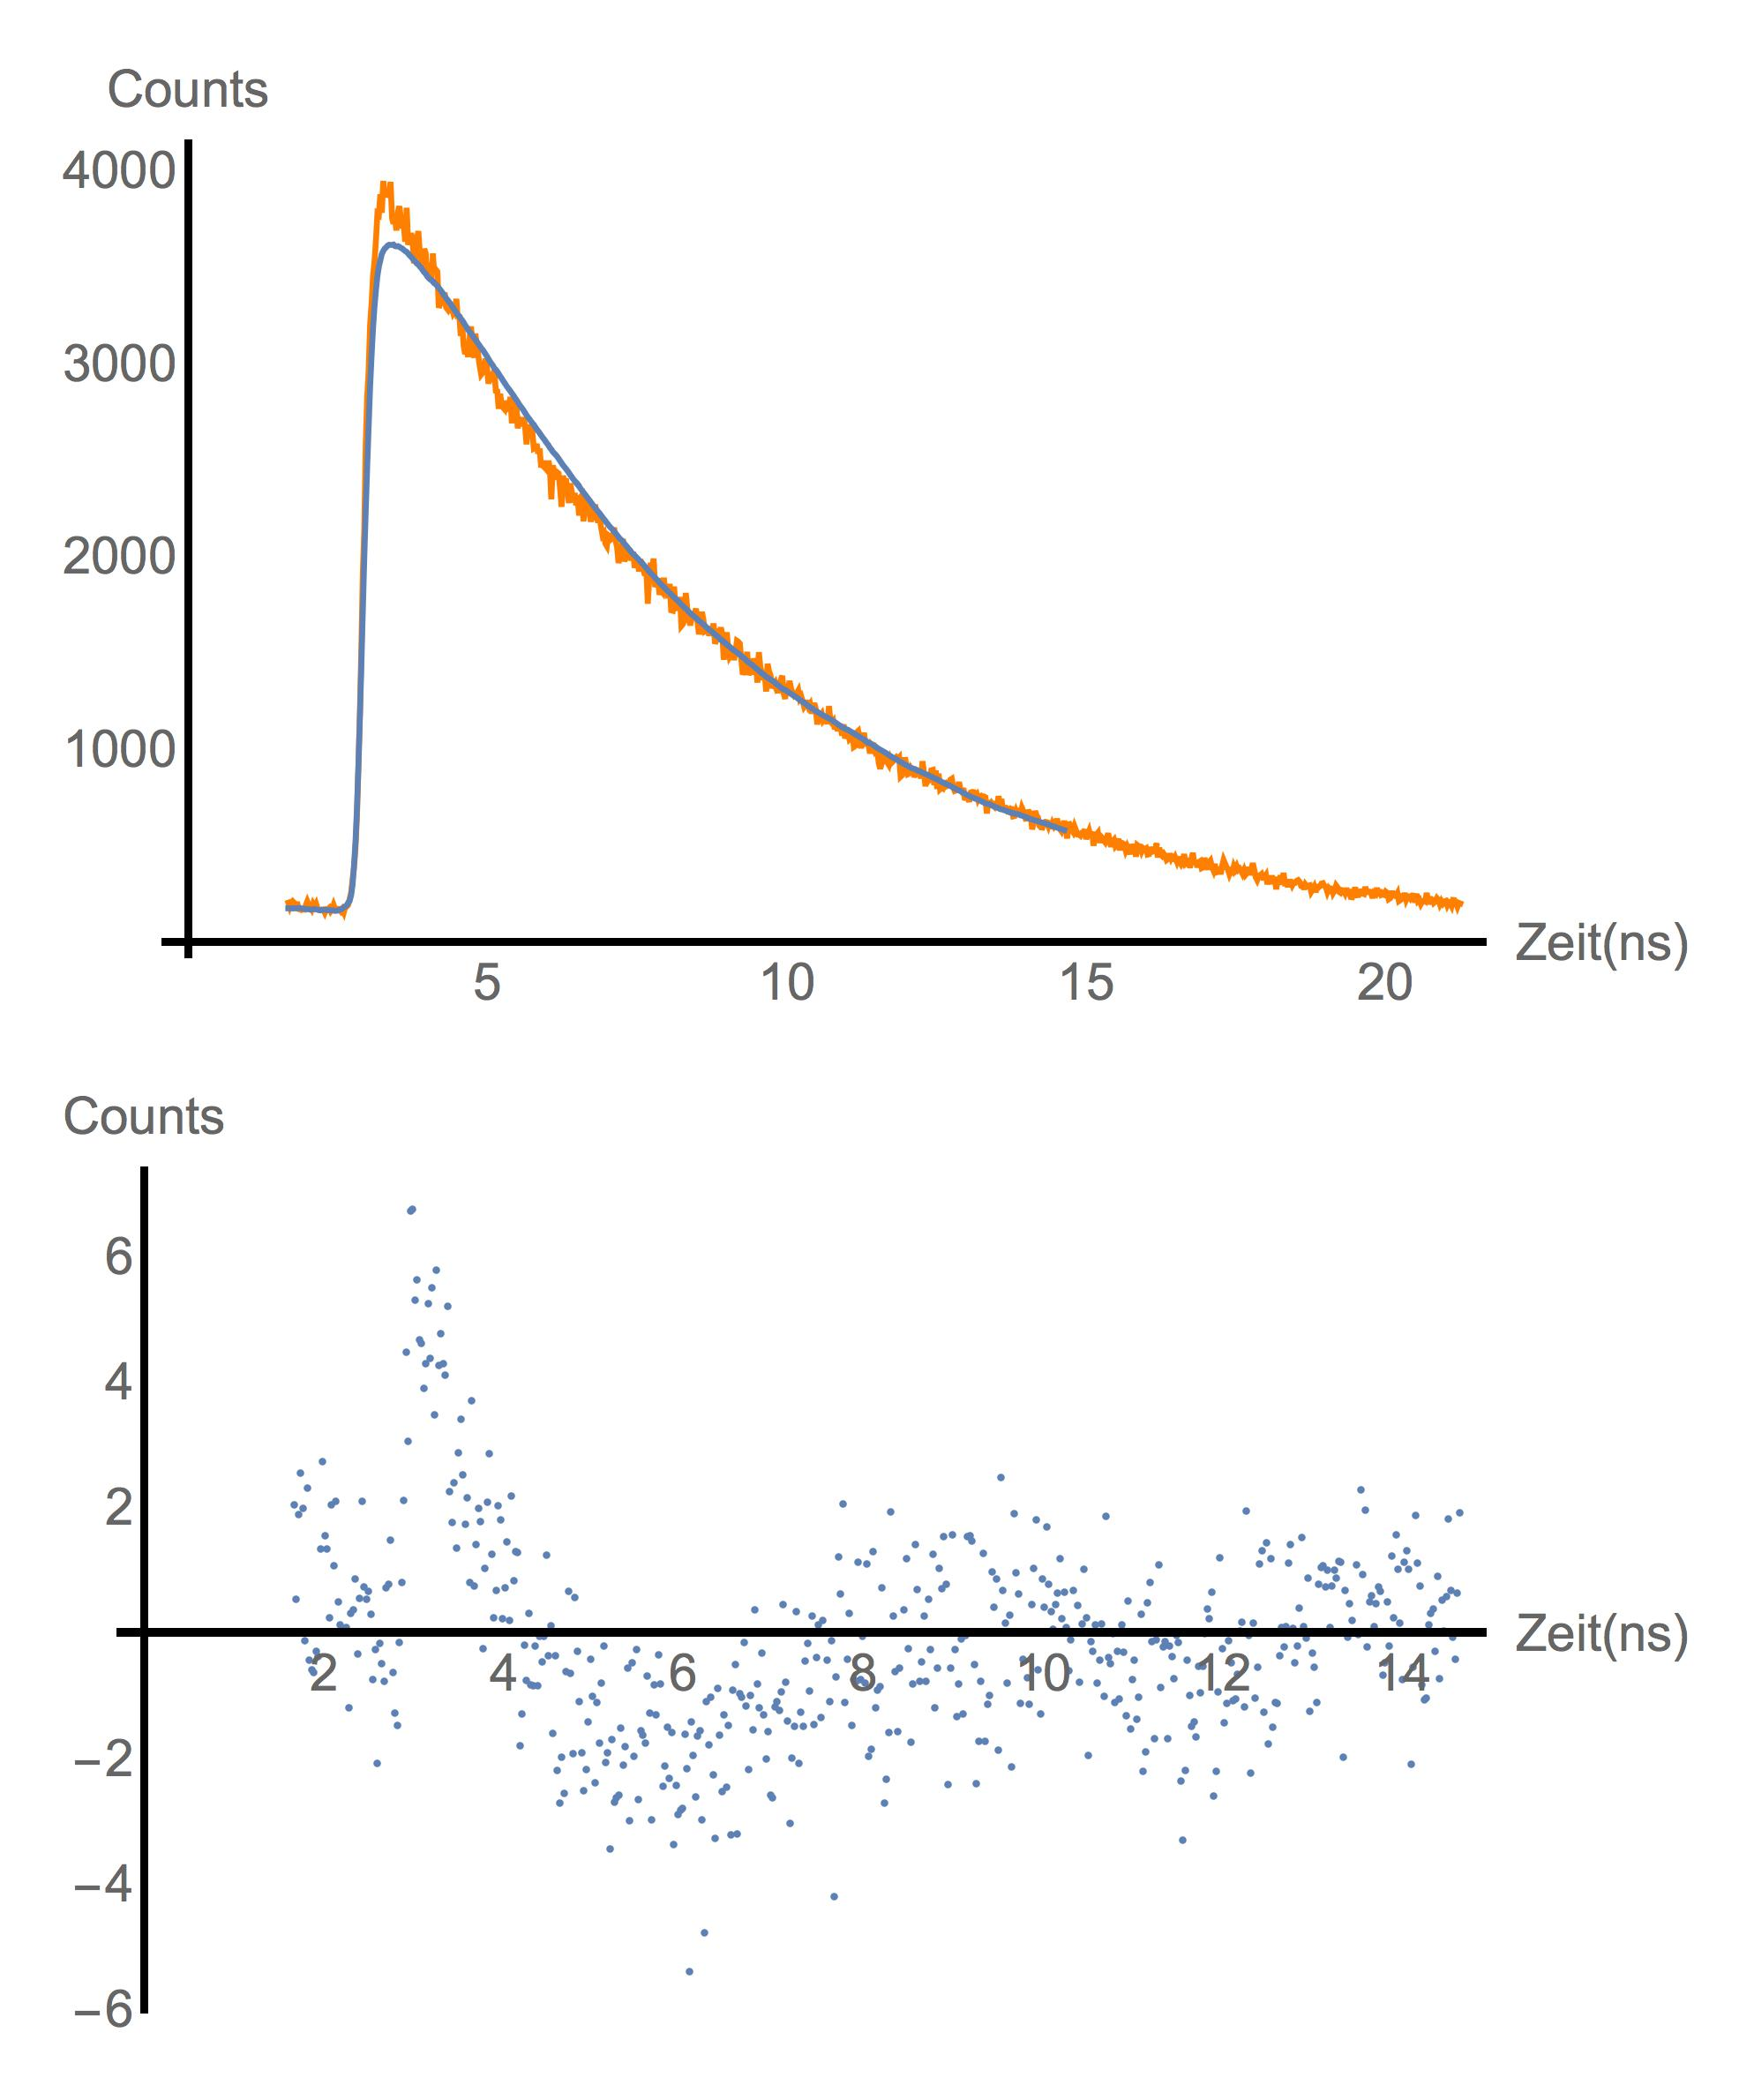
\includegraphics[width=\textwidth/2]{Bilder/FitOD03.jpg}  &   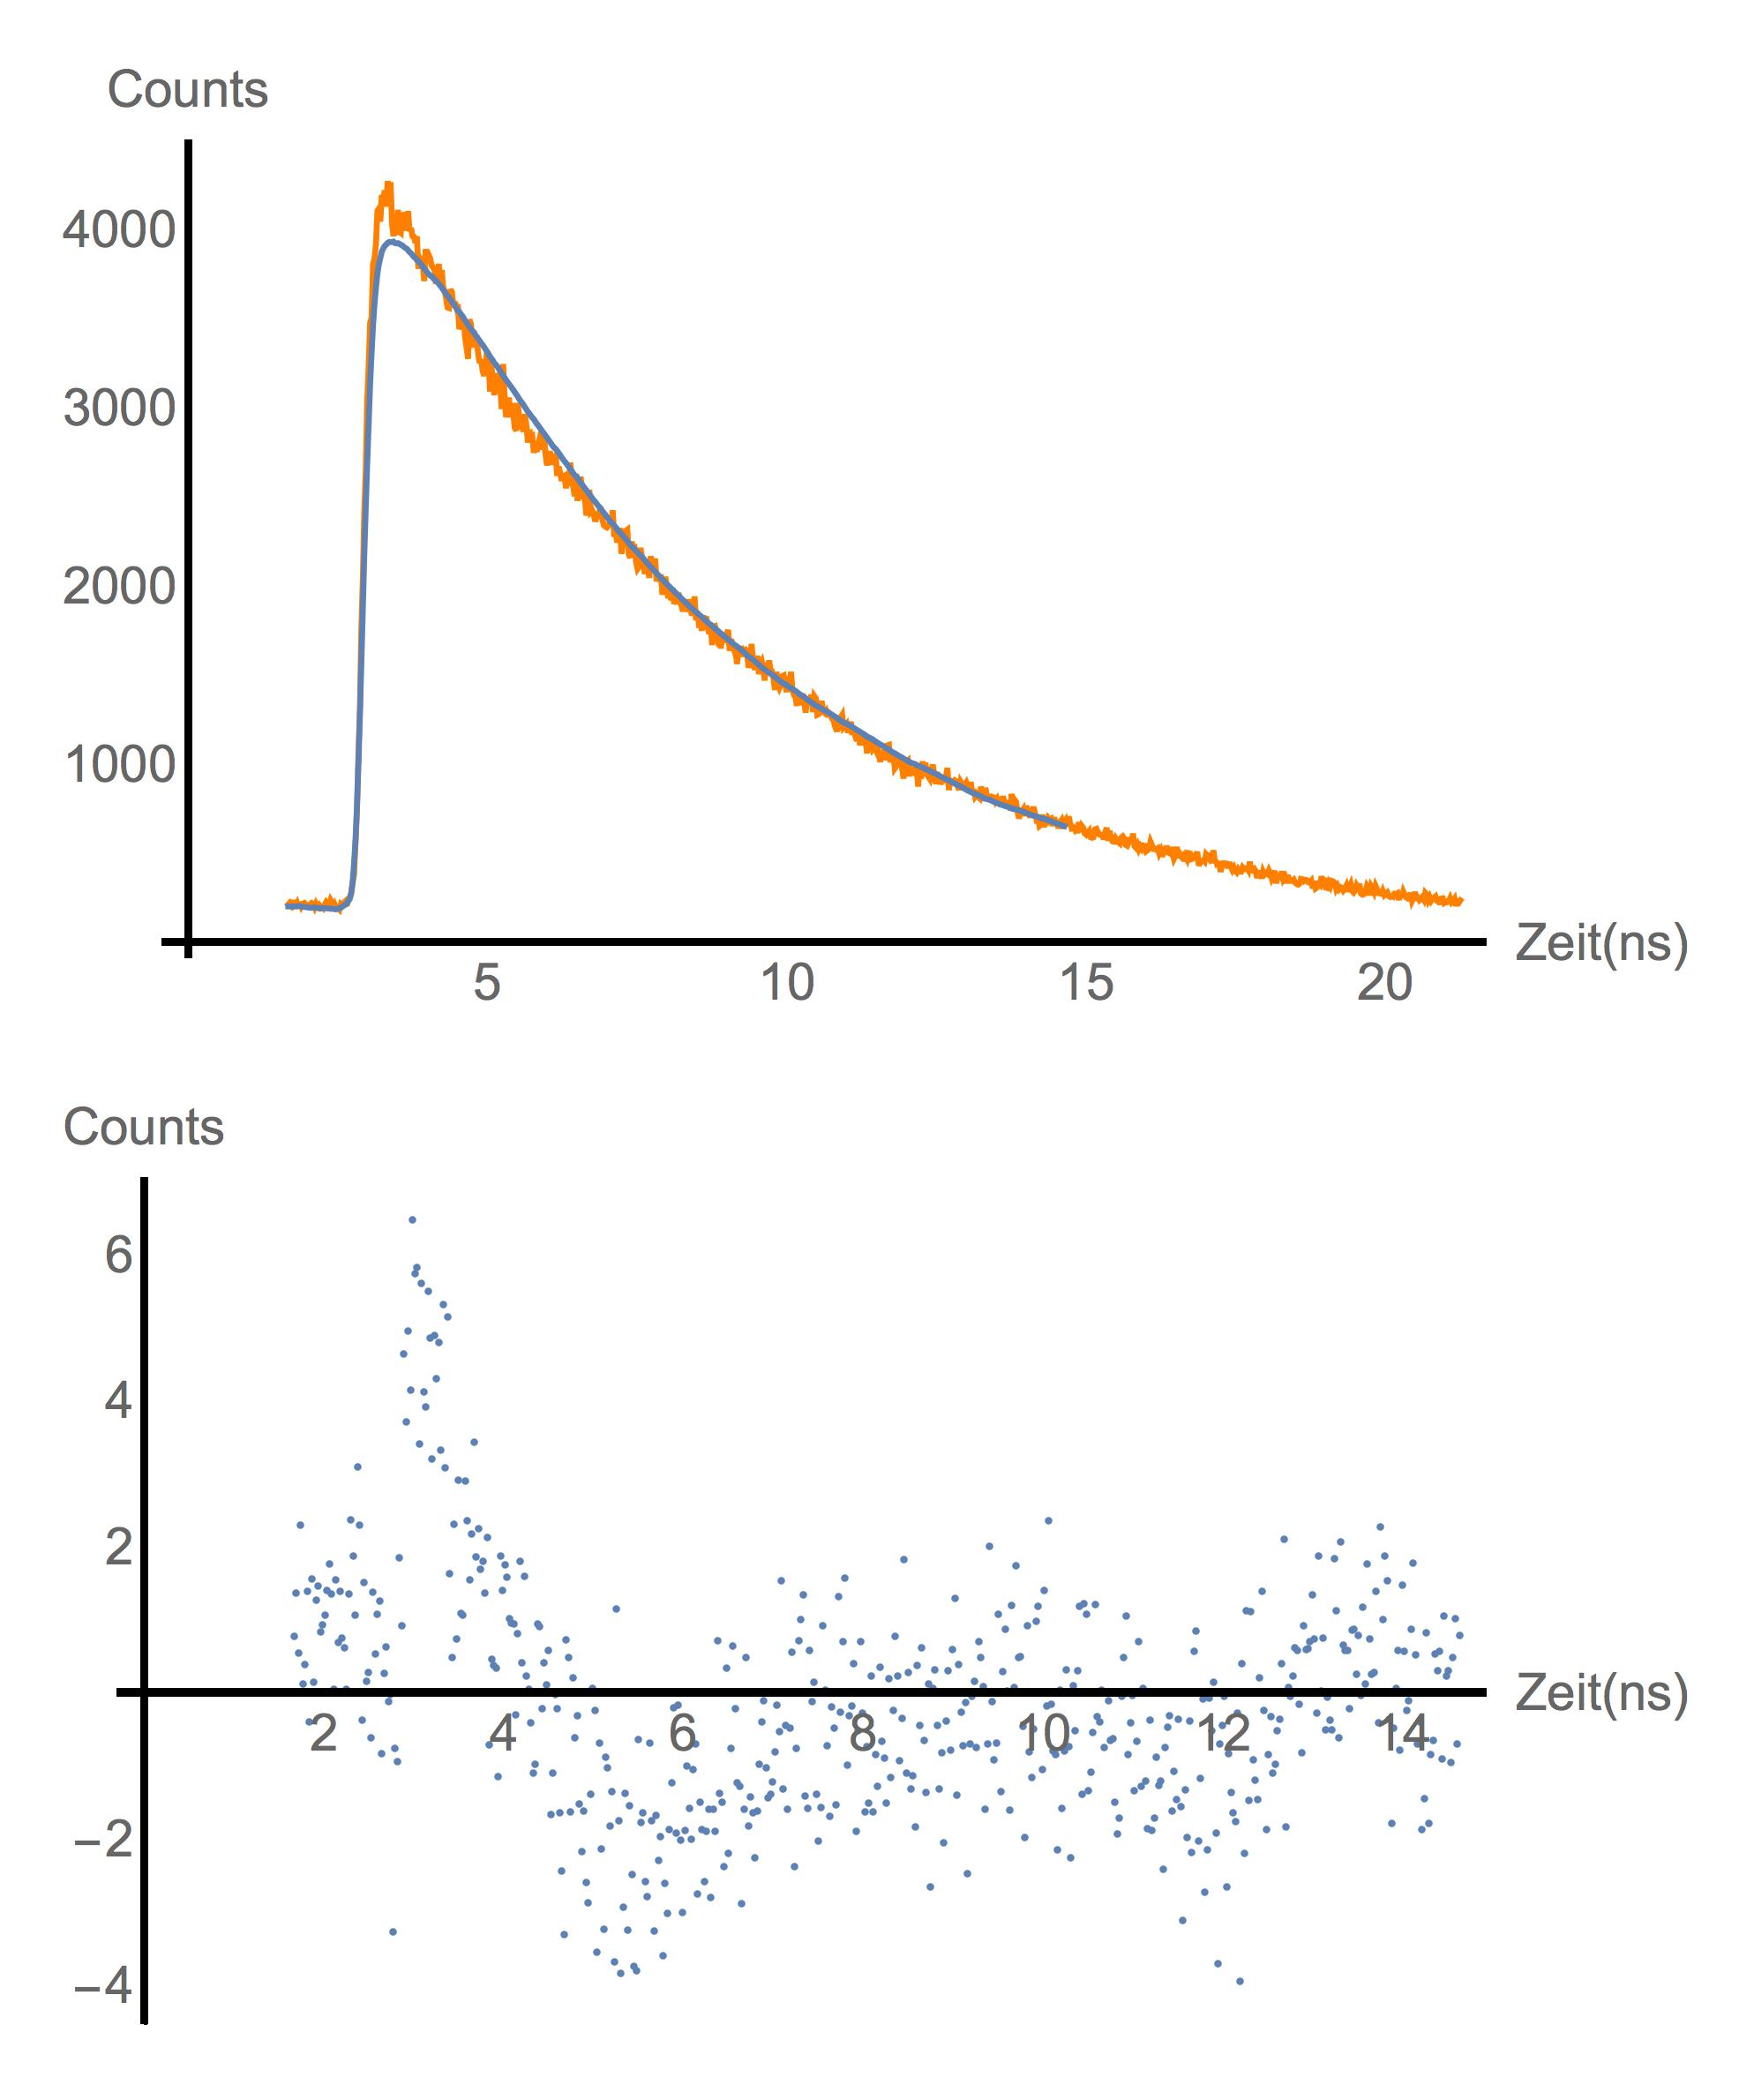
\includegraphics[width=\textwidth/2]{Bilder/FitOD07.jpg}\\
  (a) OD = 0.3, $\chi^2$=1.66                                 &   (b) OD = 0.7, $\chi^2$=1.64                               \\
  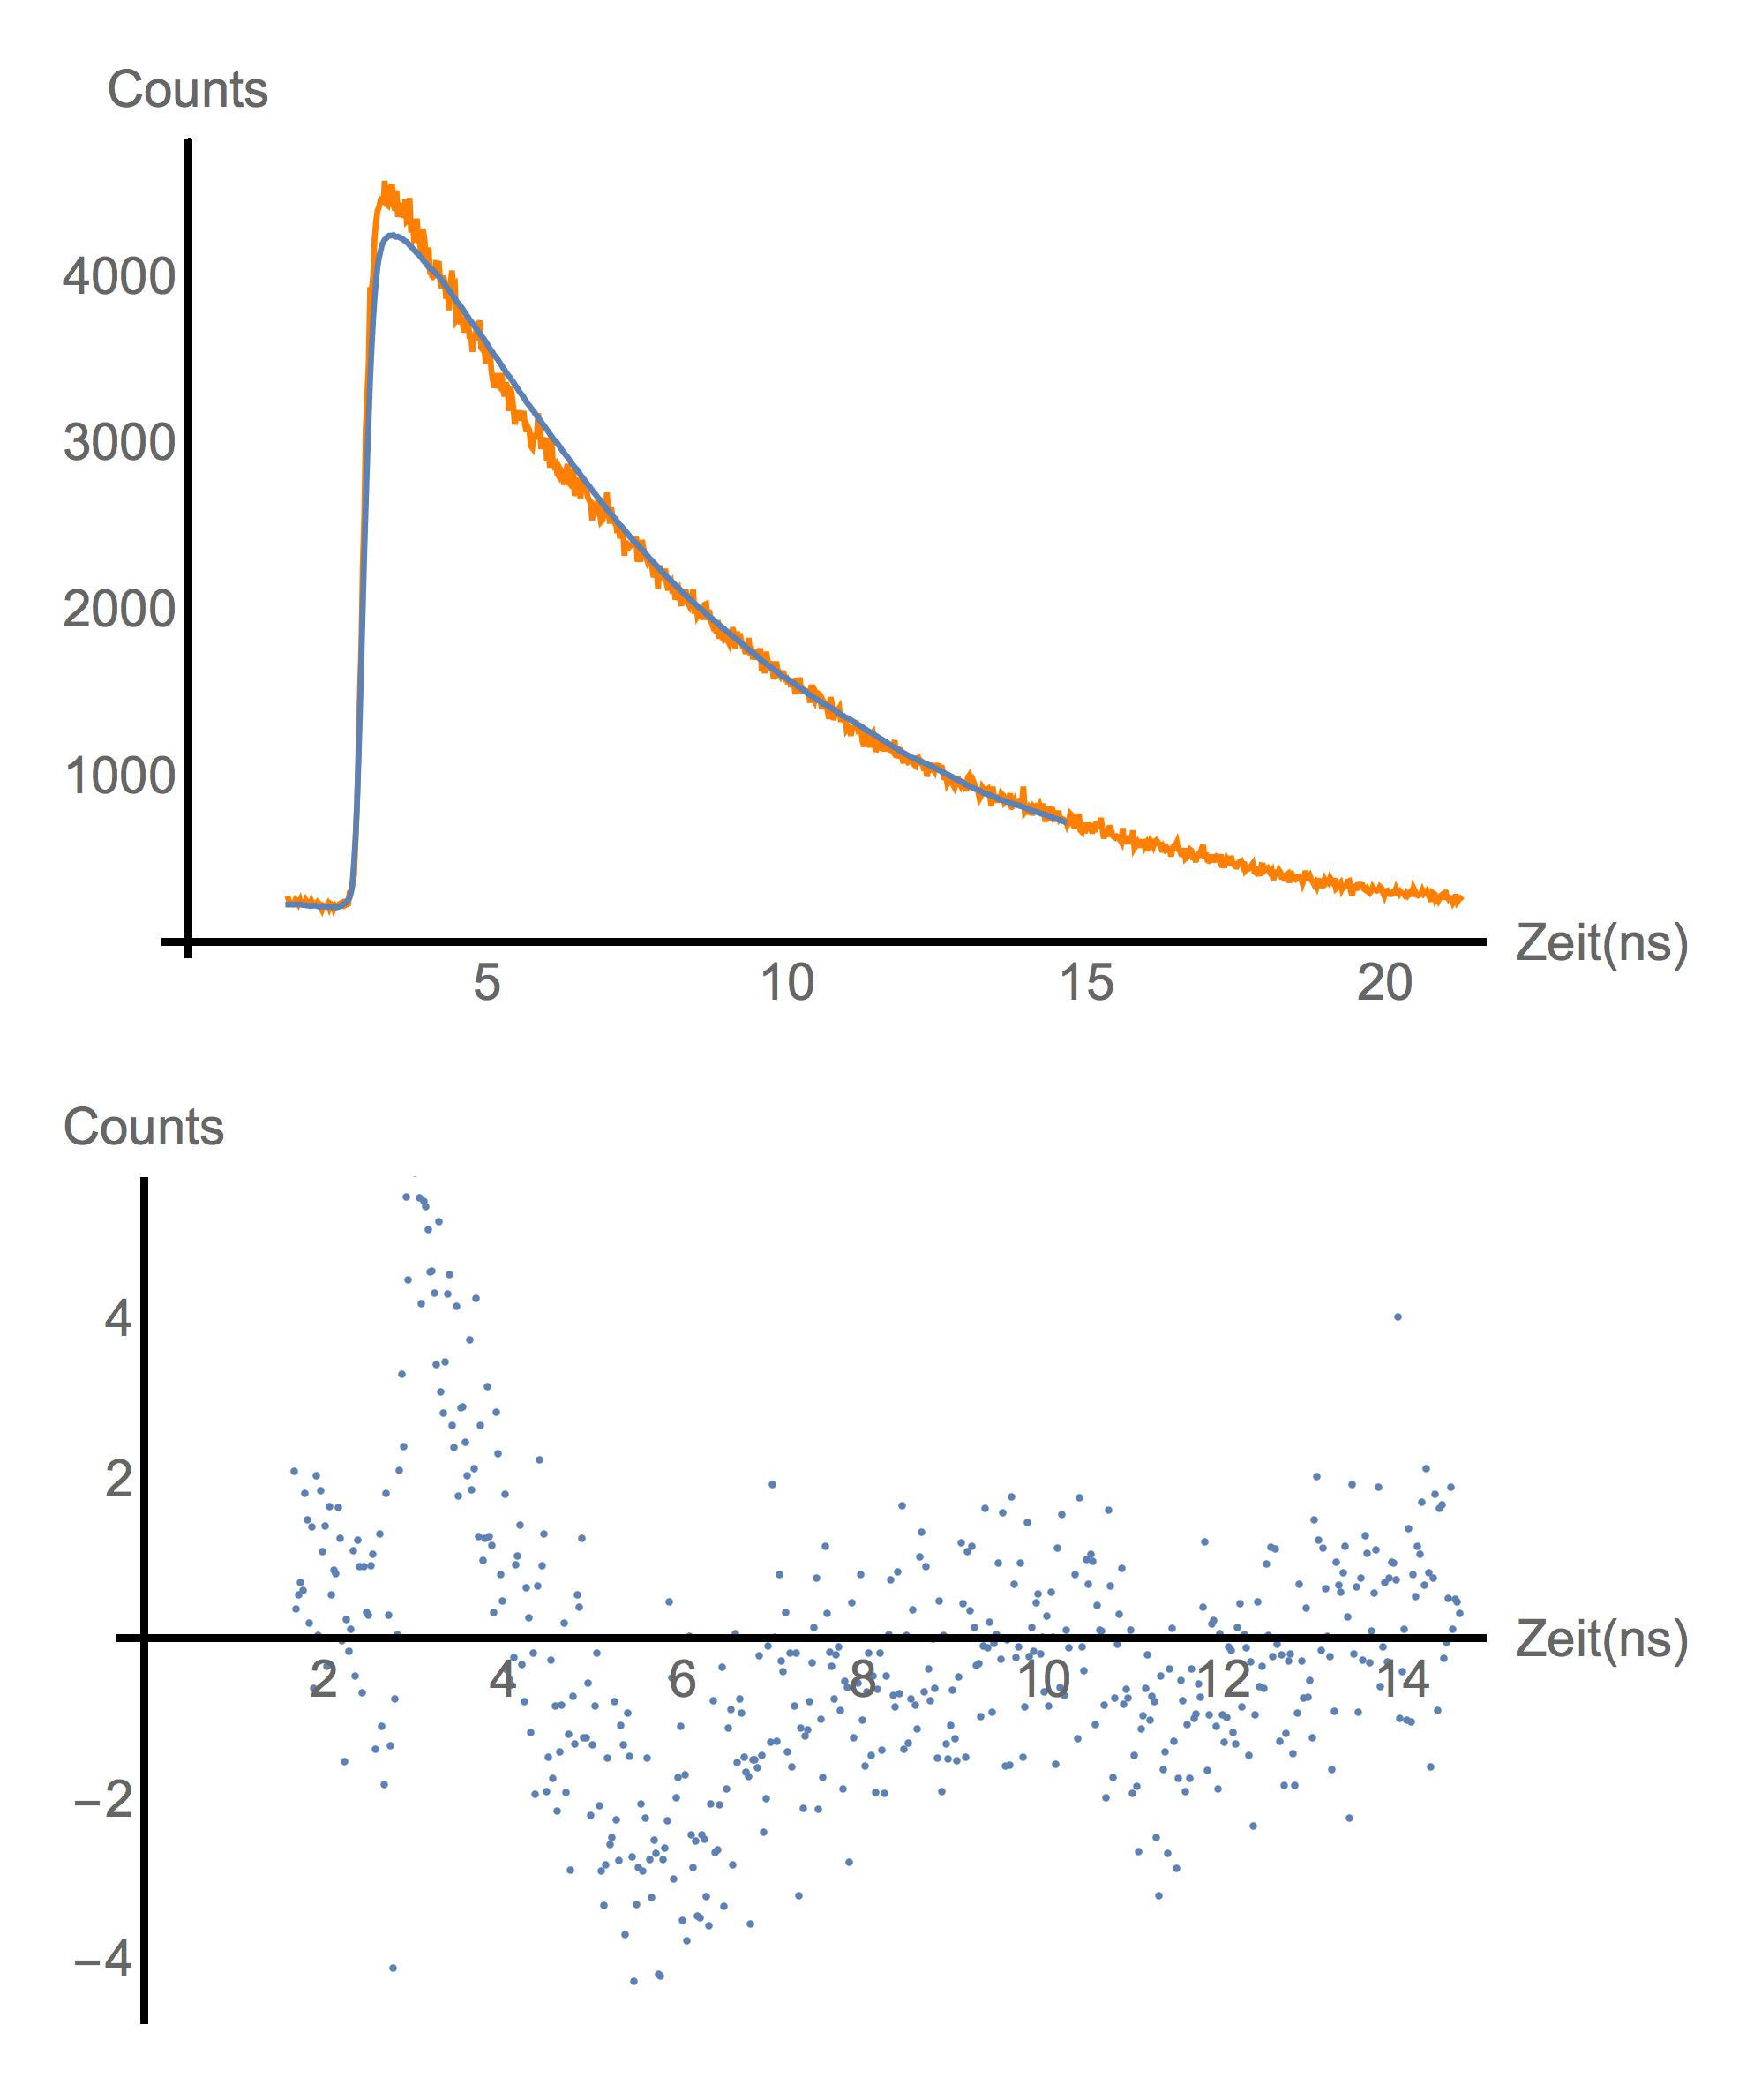
\includegraphics[width=\textwidth/2]{Bilder/FitOD11.jpg}  &   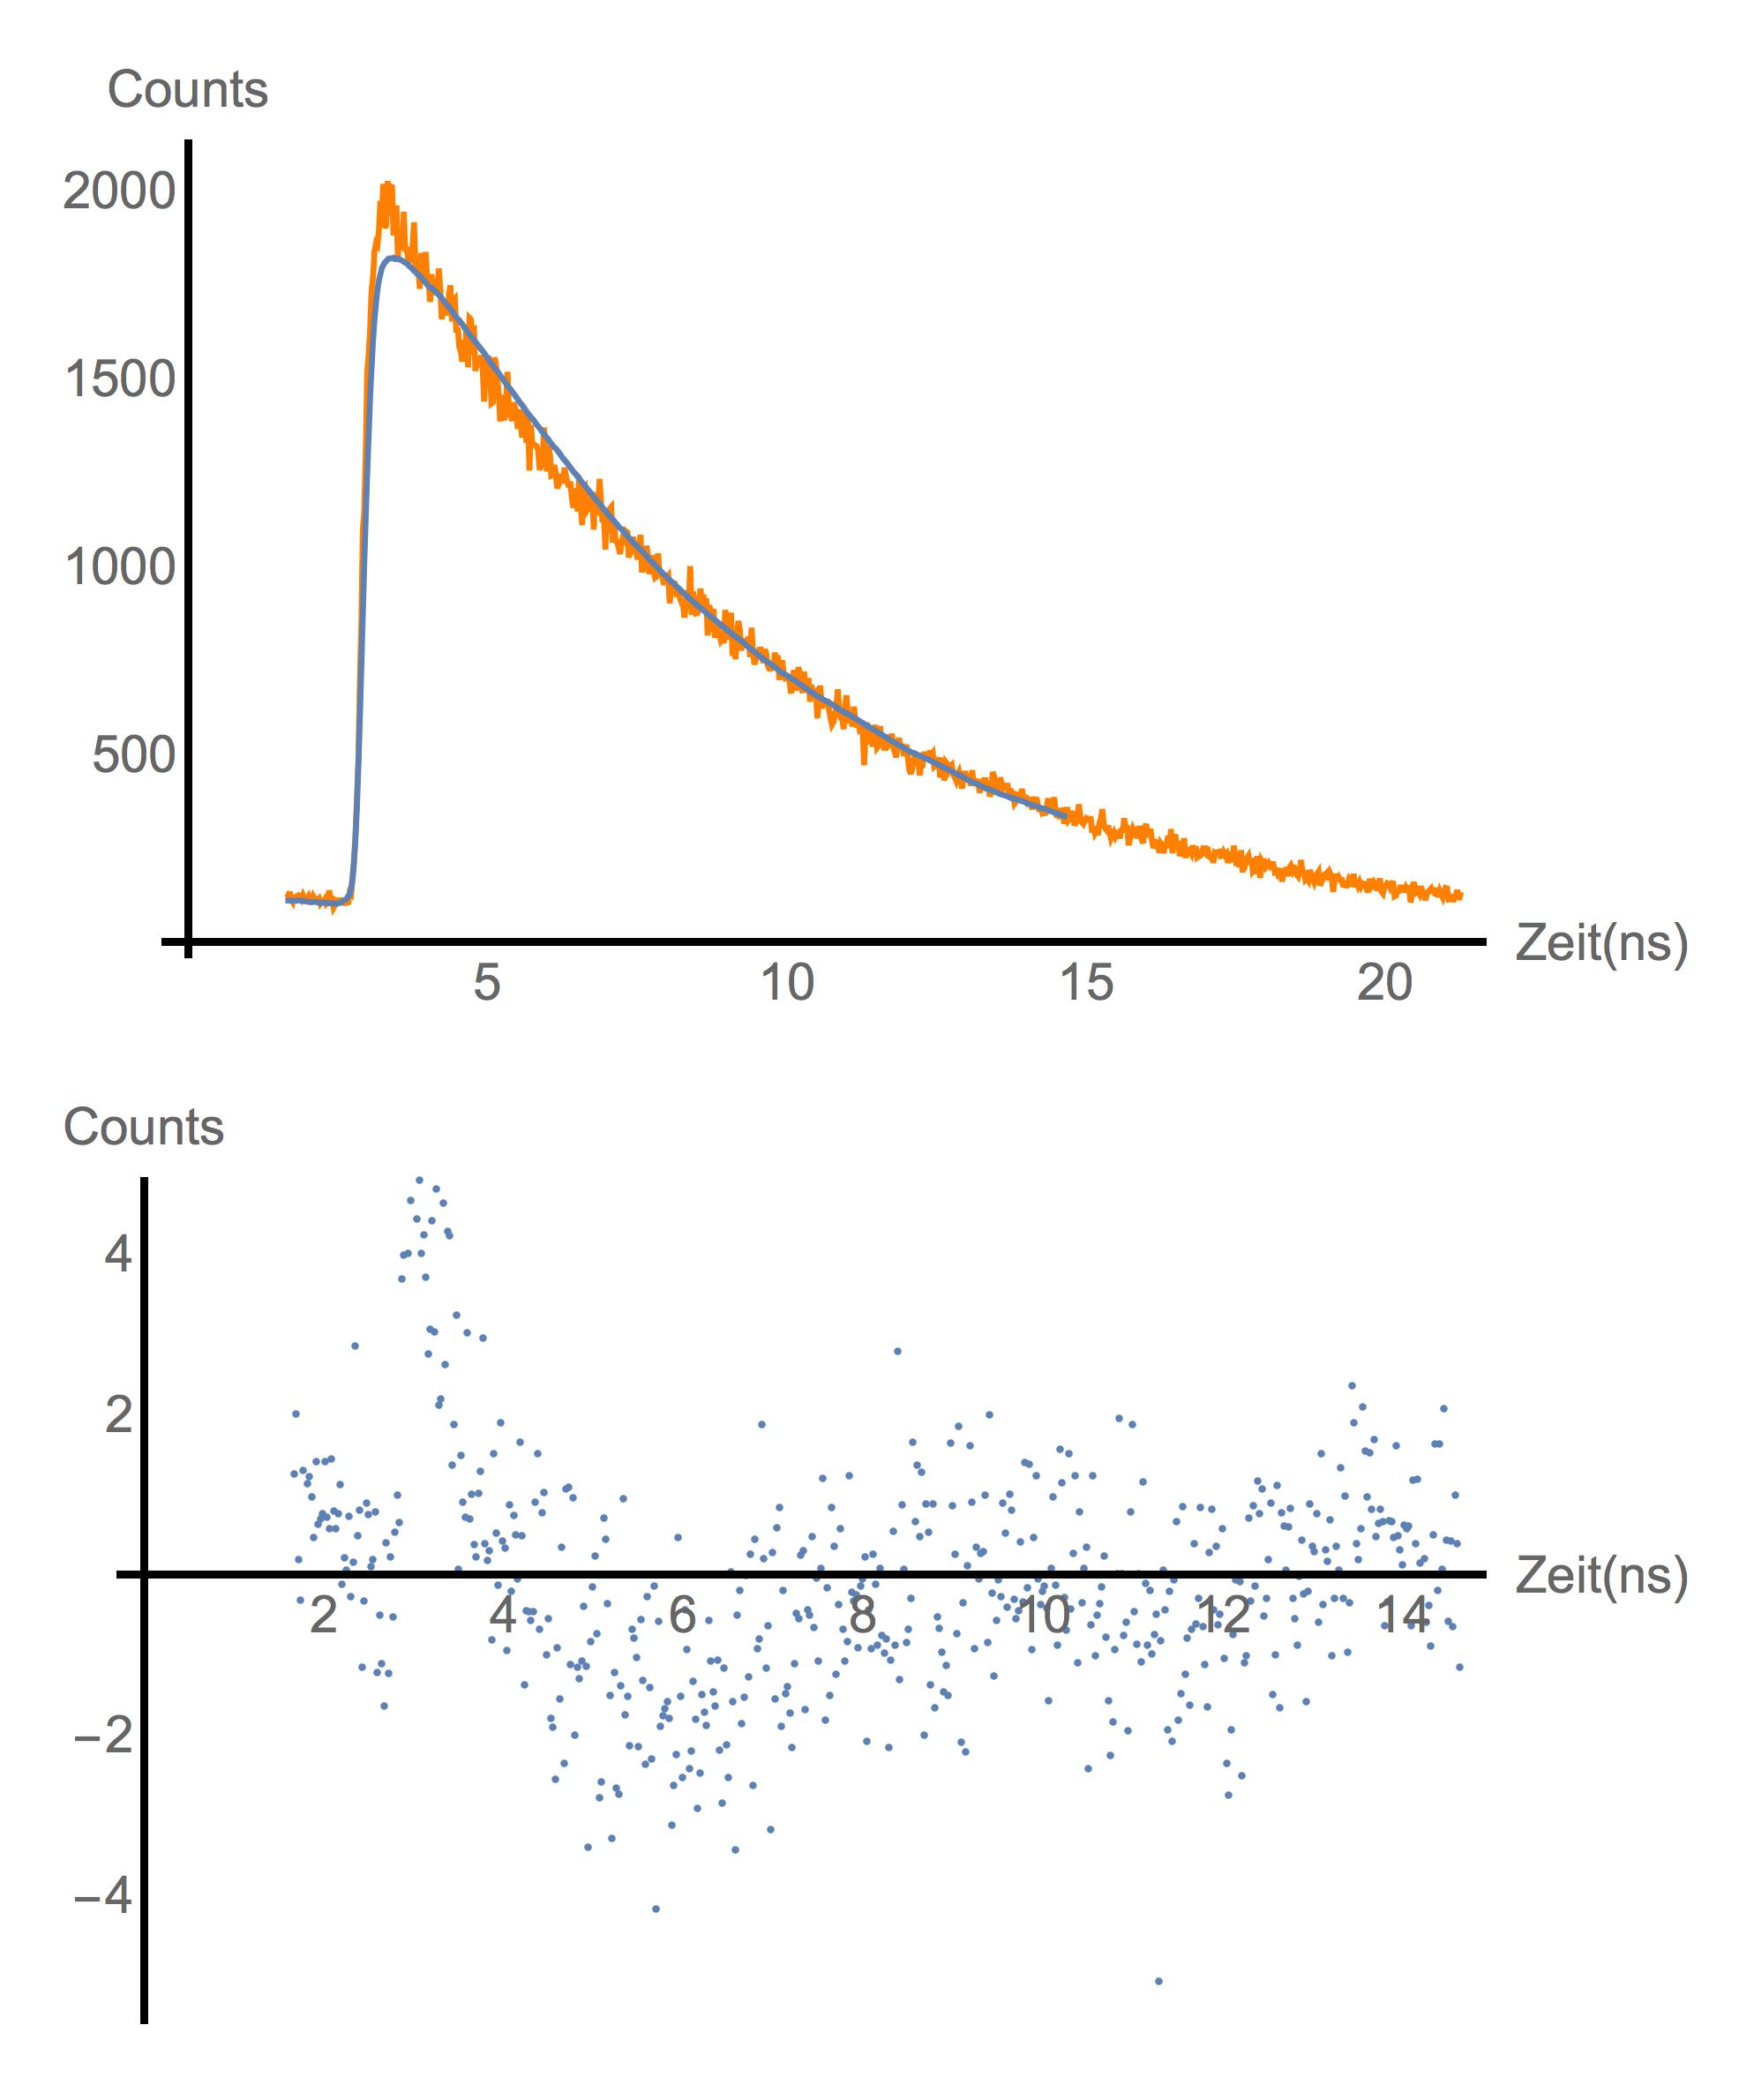
\includegraphics[width=\textwidth/2]{Bilder/FitOD15.jpg}\\
  (c) OD = 1.1, $\chi^2$=1.79                                 &   (d) OD = 1.5, $\chi^2$=1.50                               \\

\end{tabular}
\caption{Fits und Residuen des Reabsorptionseffekt}
\end{figure}


\begin{figure}
\begin{tabular}{cc}
  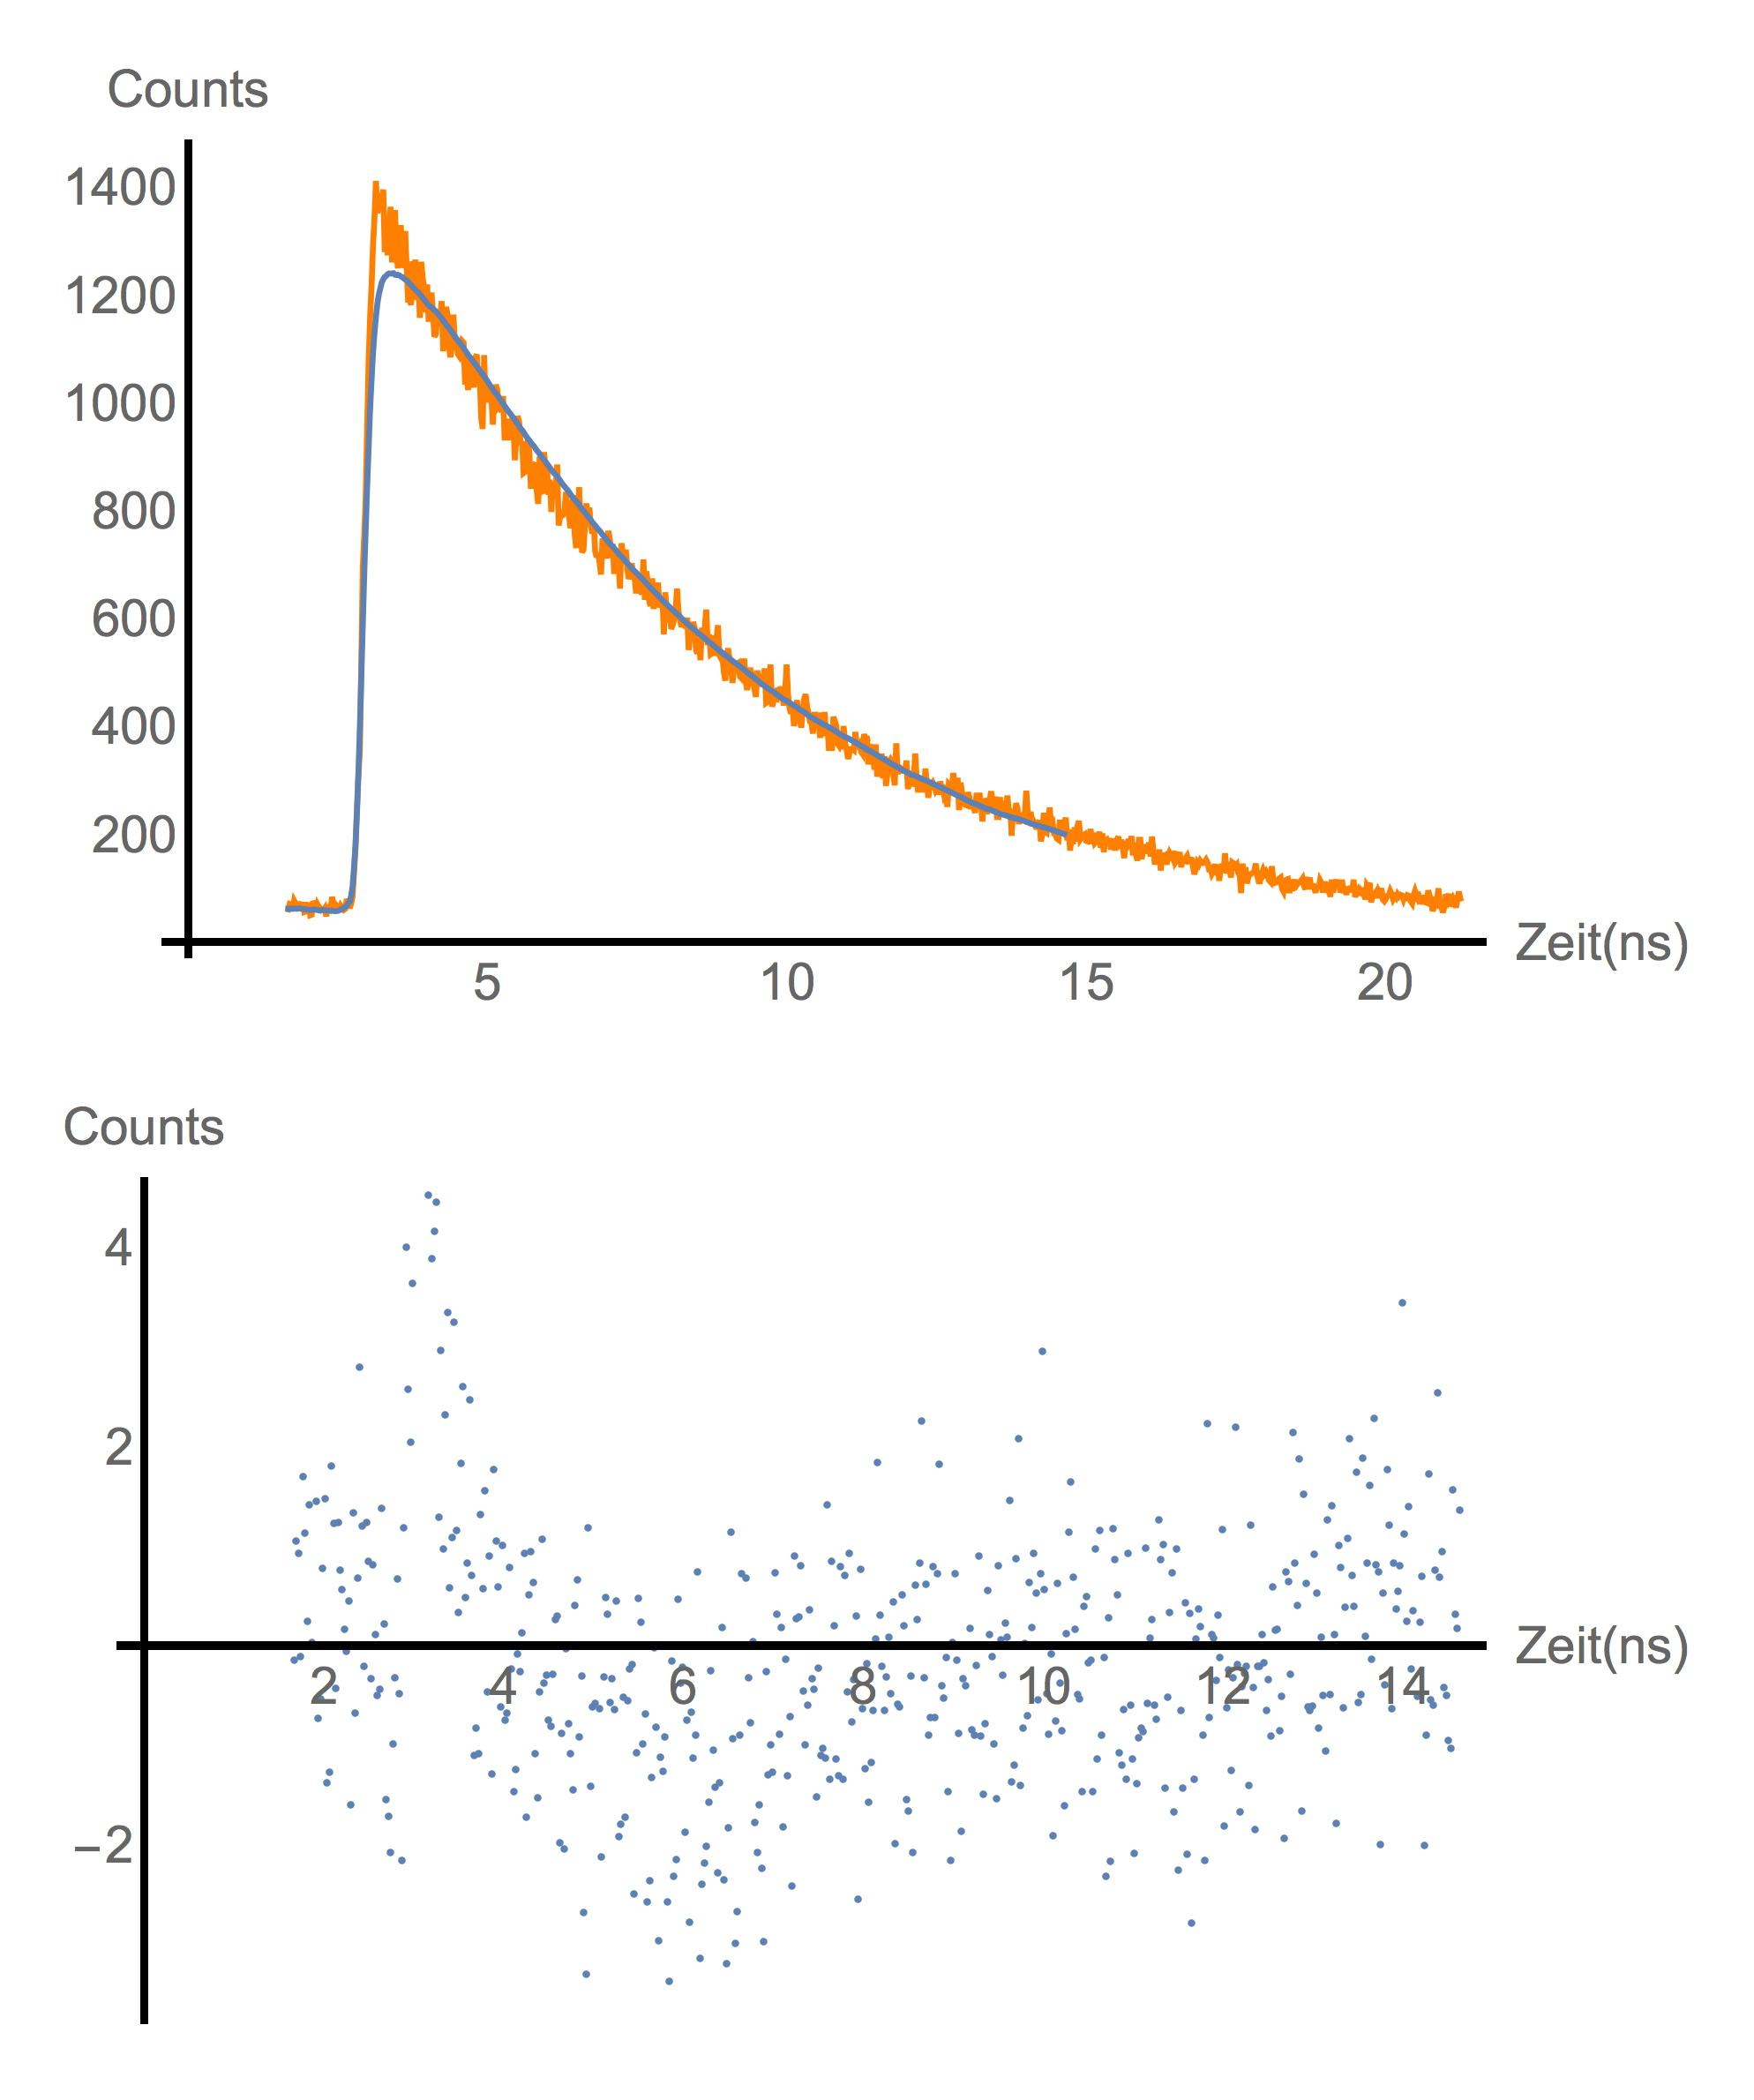
\includegraphics[width=\textwidth/2]{Bilder/Fit1509uW.jpg}  &   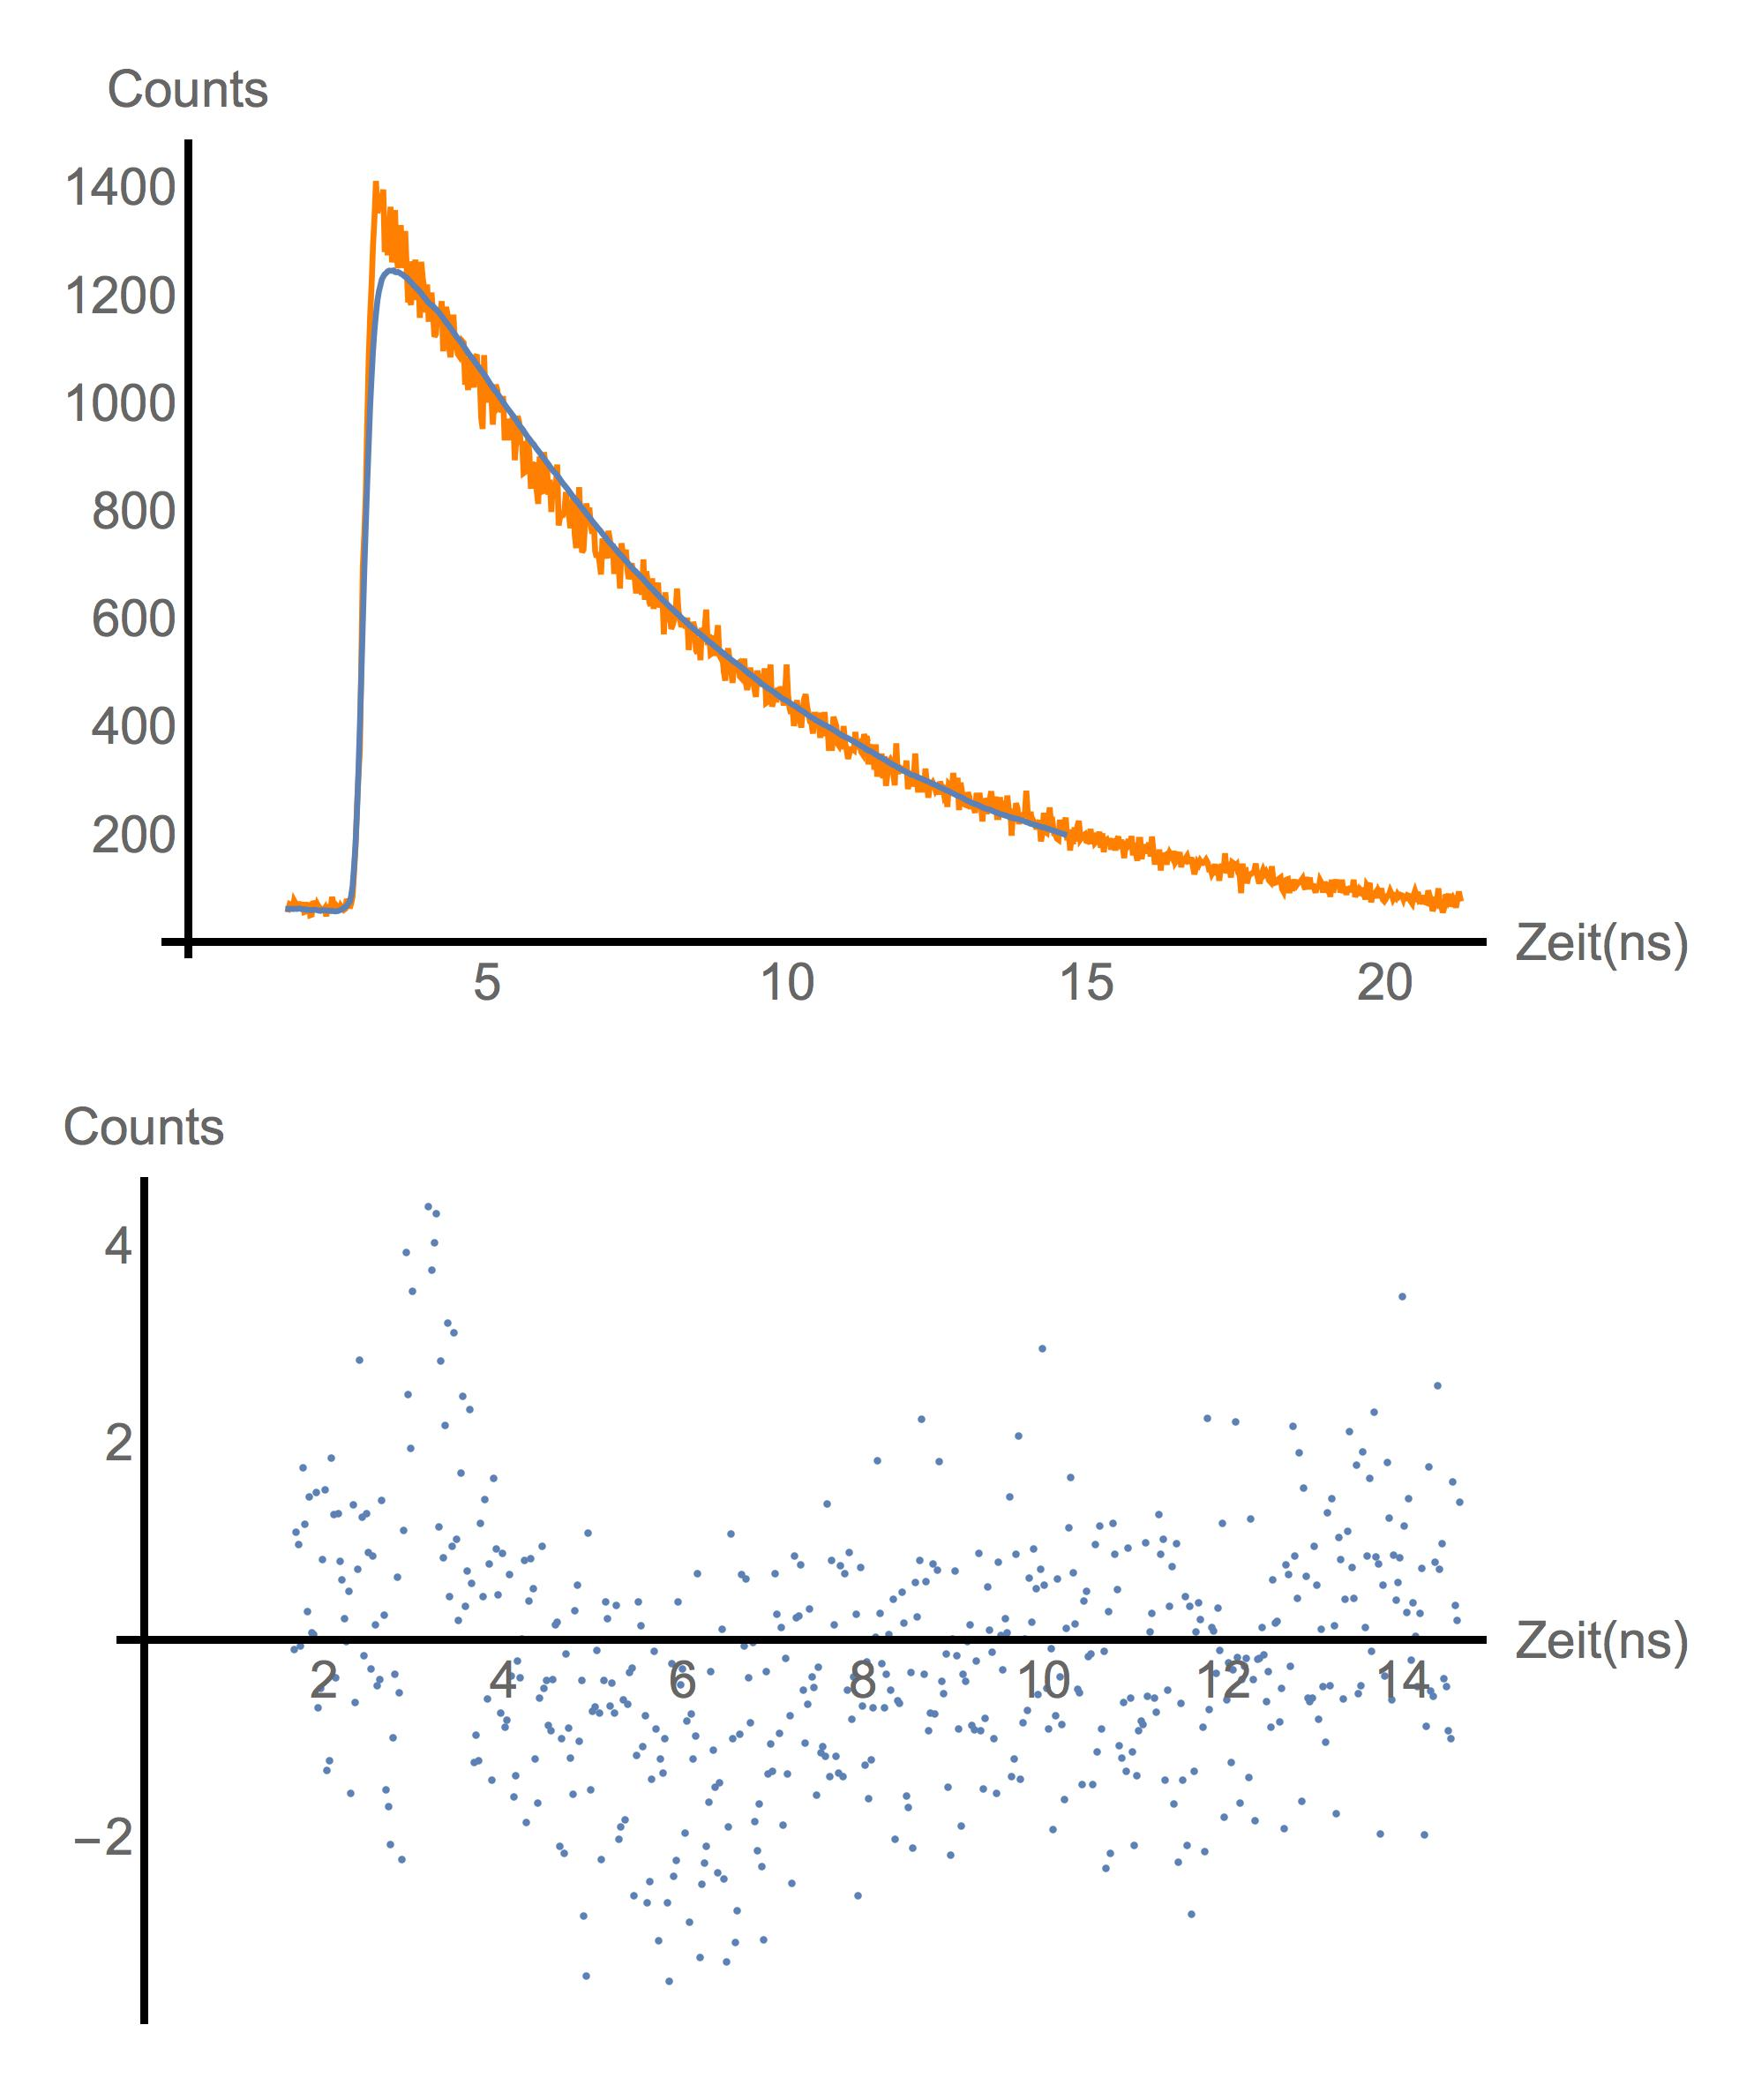
\includegraphics[width=\textwidth/2]{Bilder/Fit7700uW.jpg}\\
  (a) I = 15.09 $\mu$W, $\chi^2$=1.42                            &   (b) I = 77 $\mu$W, $\chi^2$=1.42                             \\
  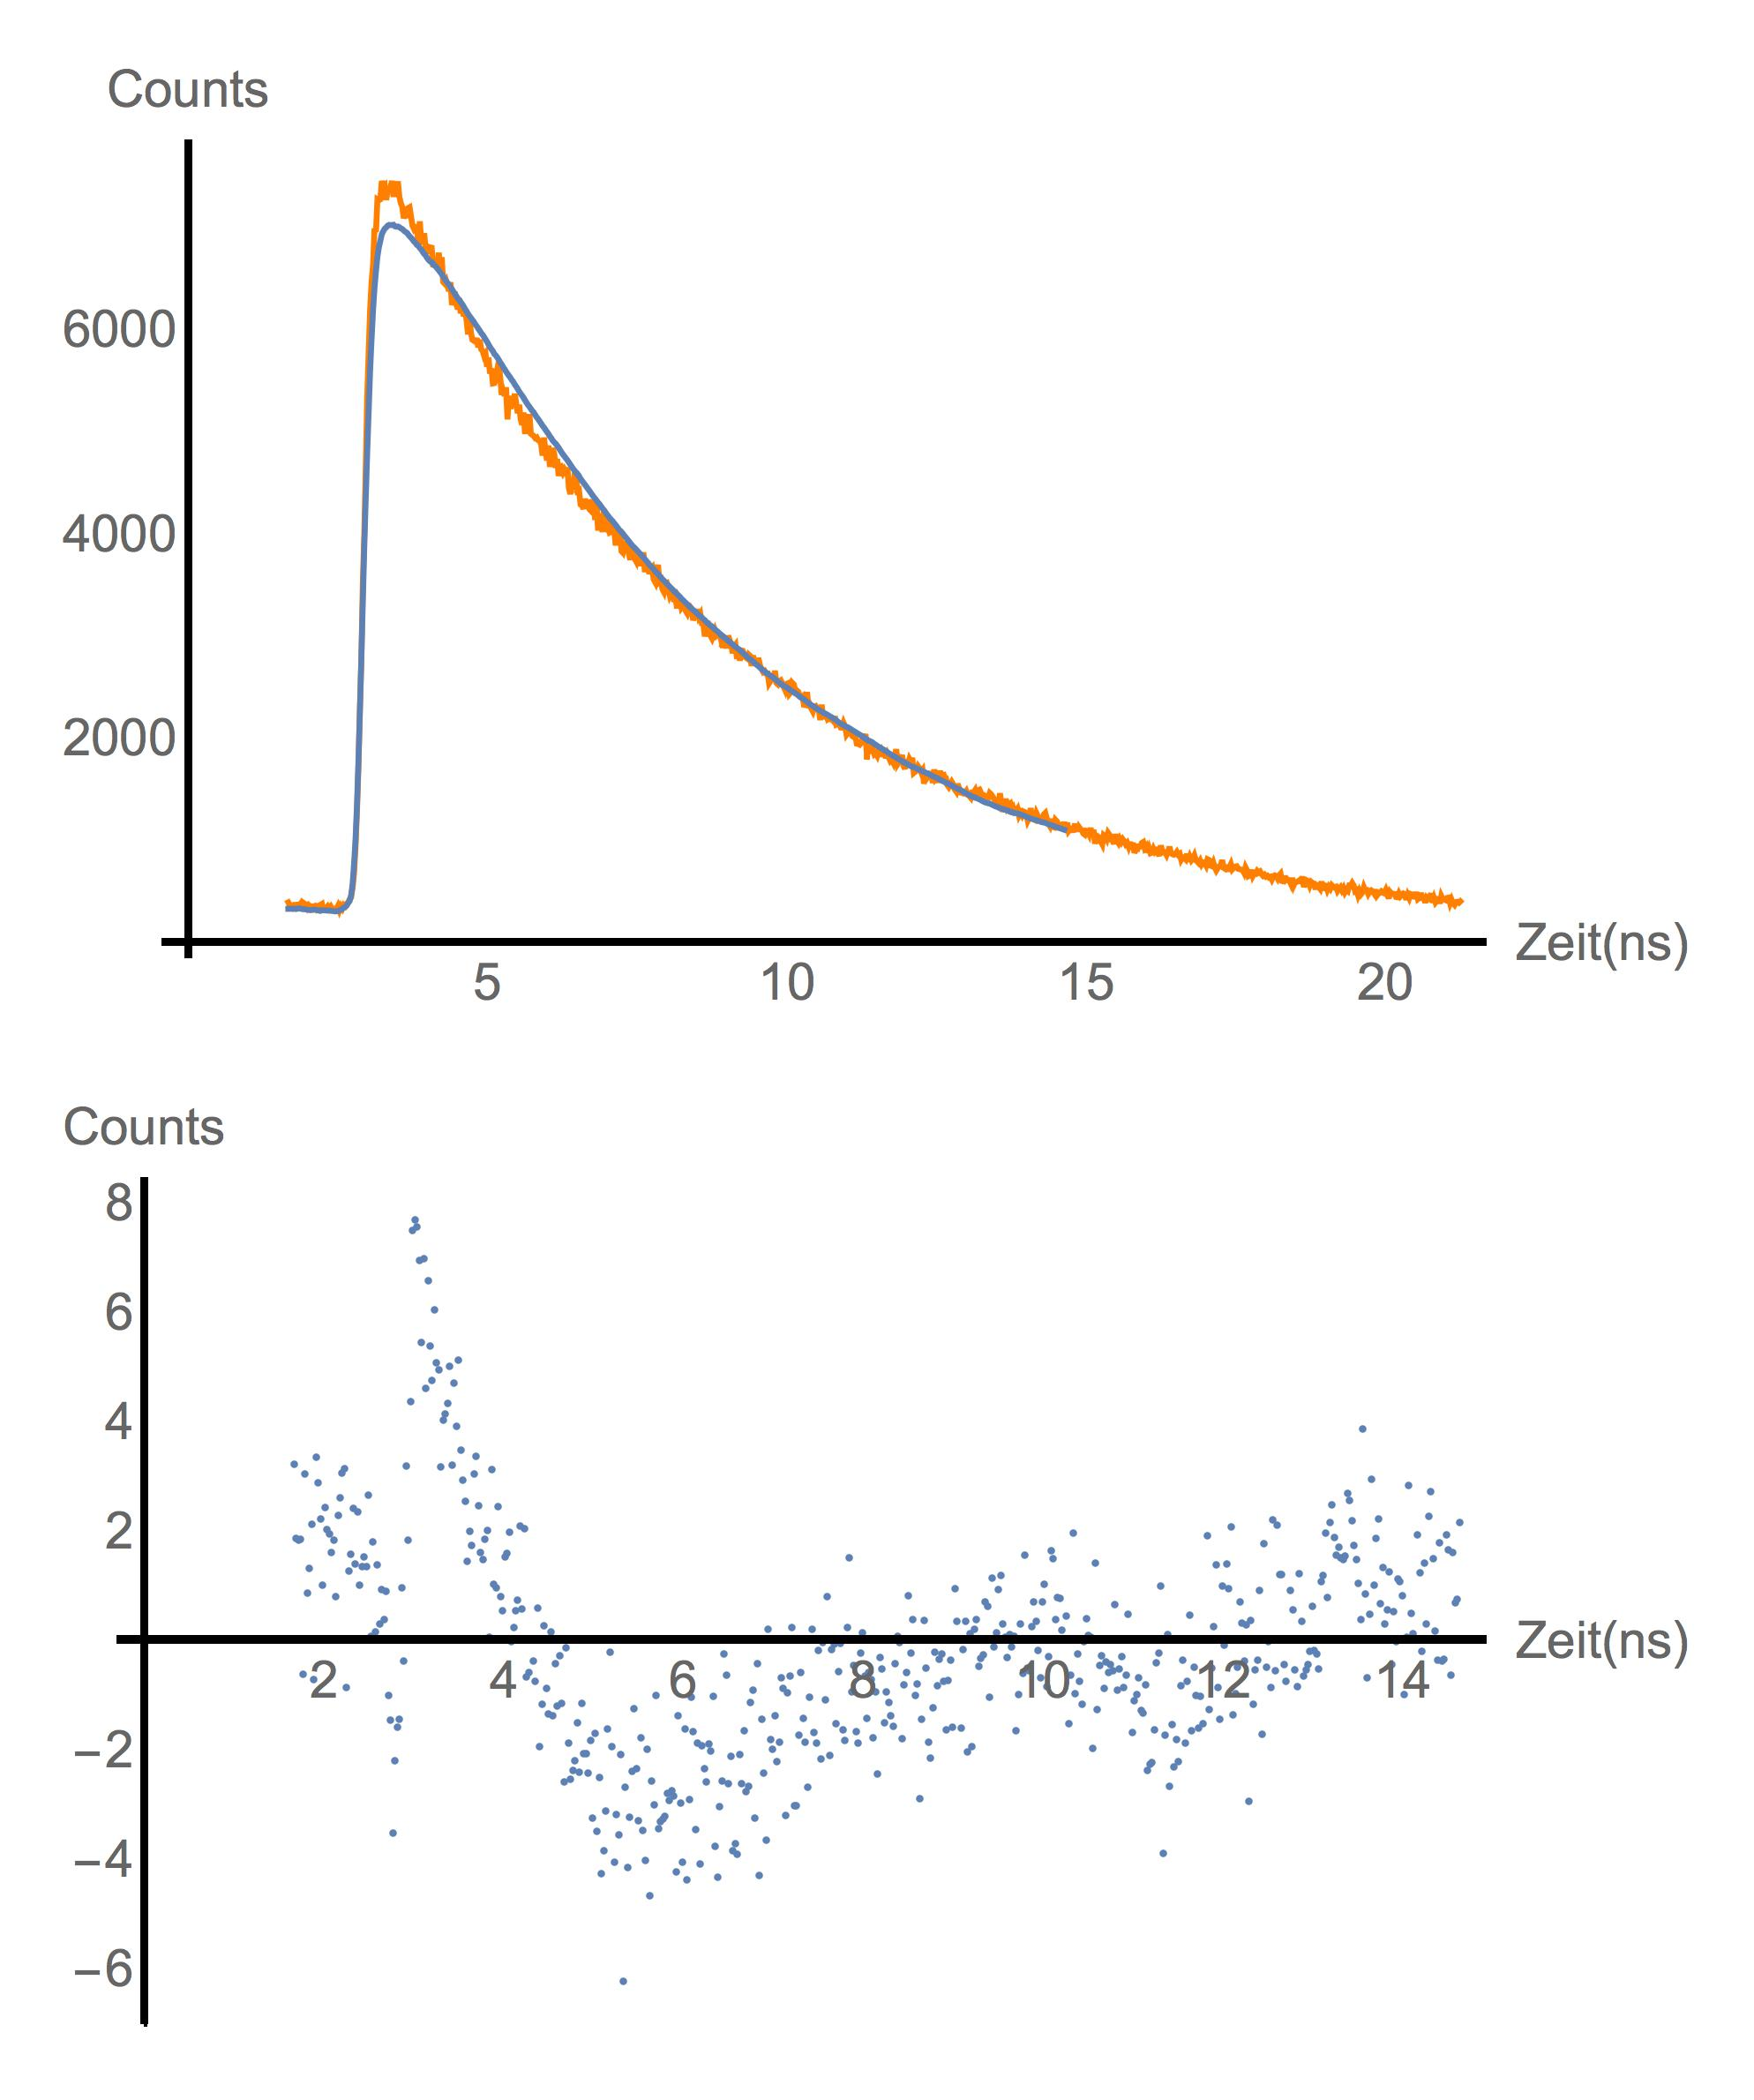
\includegraphics[width=\textwidth/2]{Bilder/Fit7900uW.jpg}  &   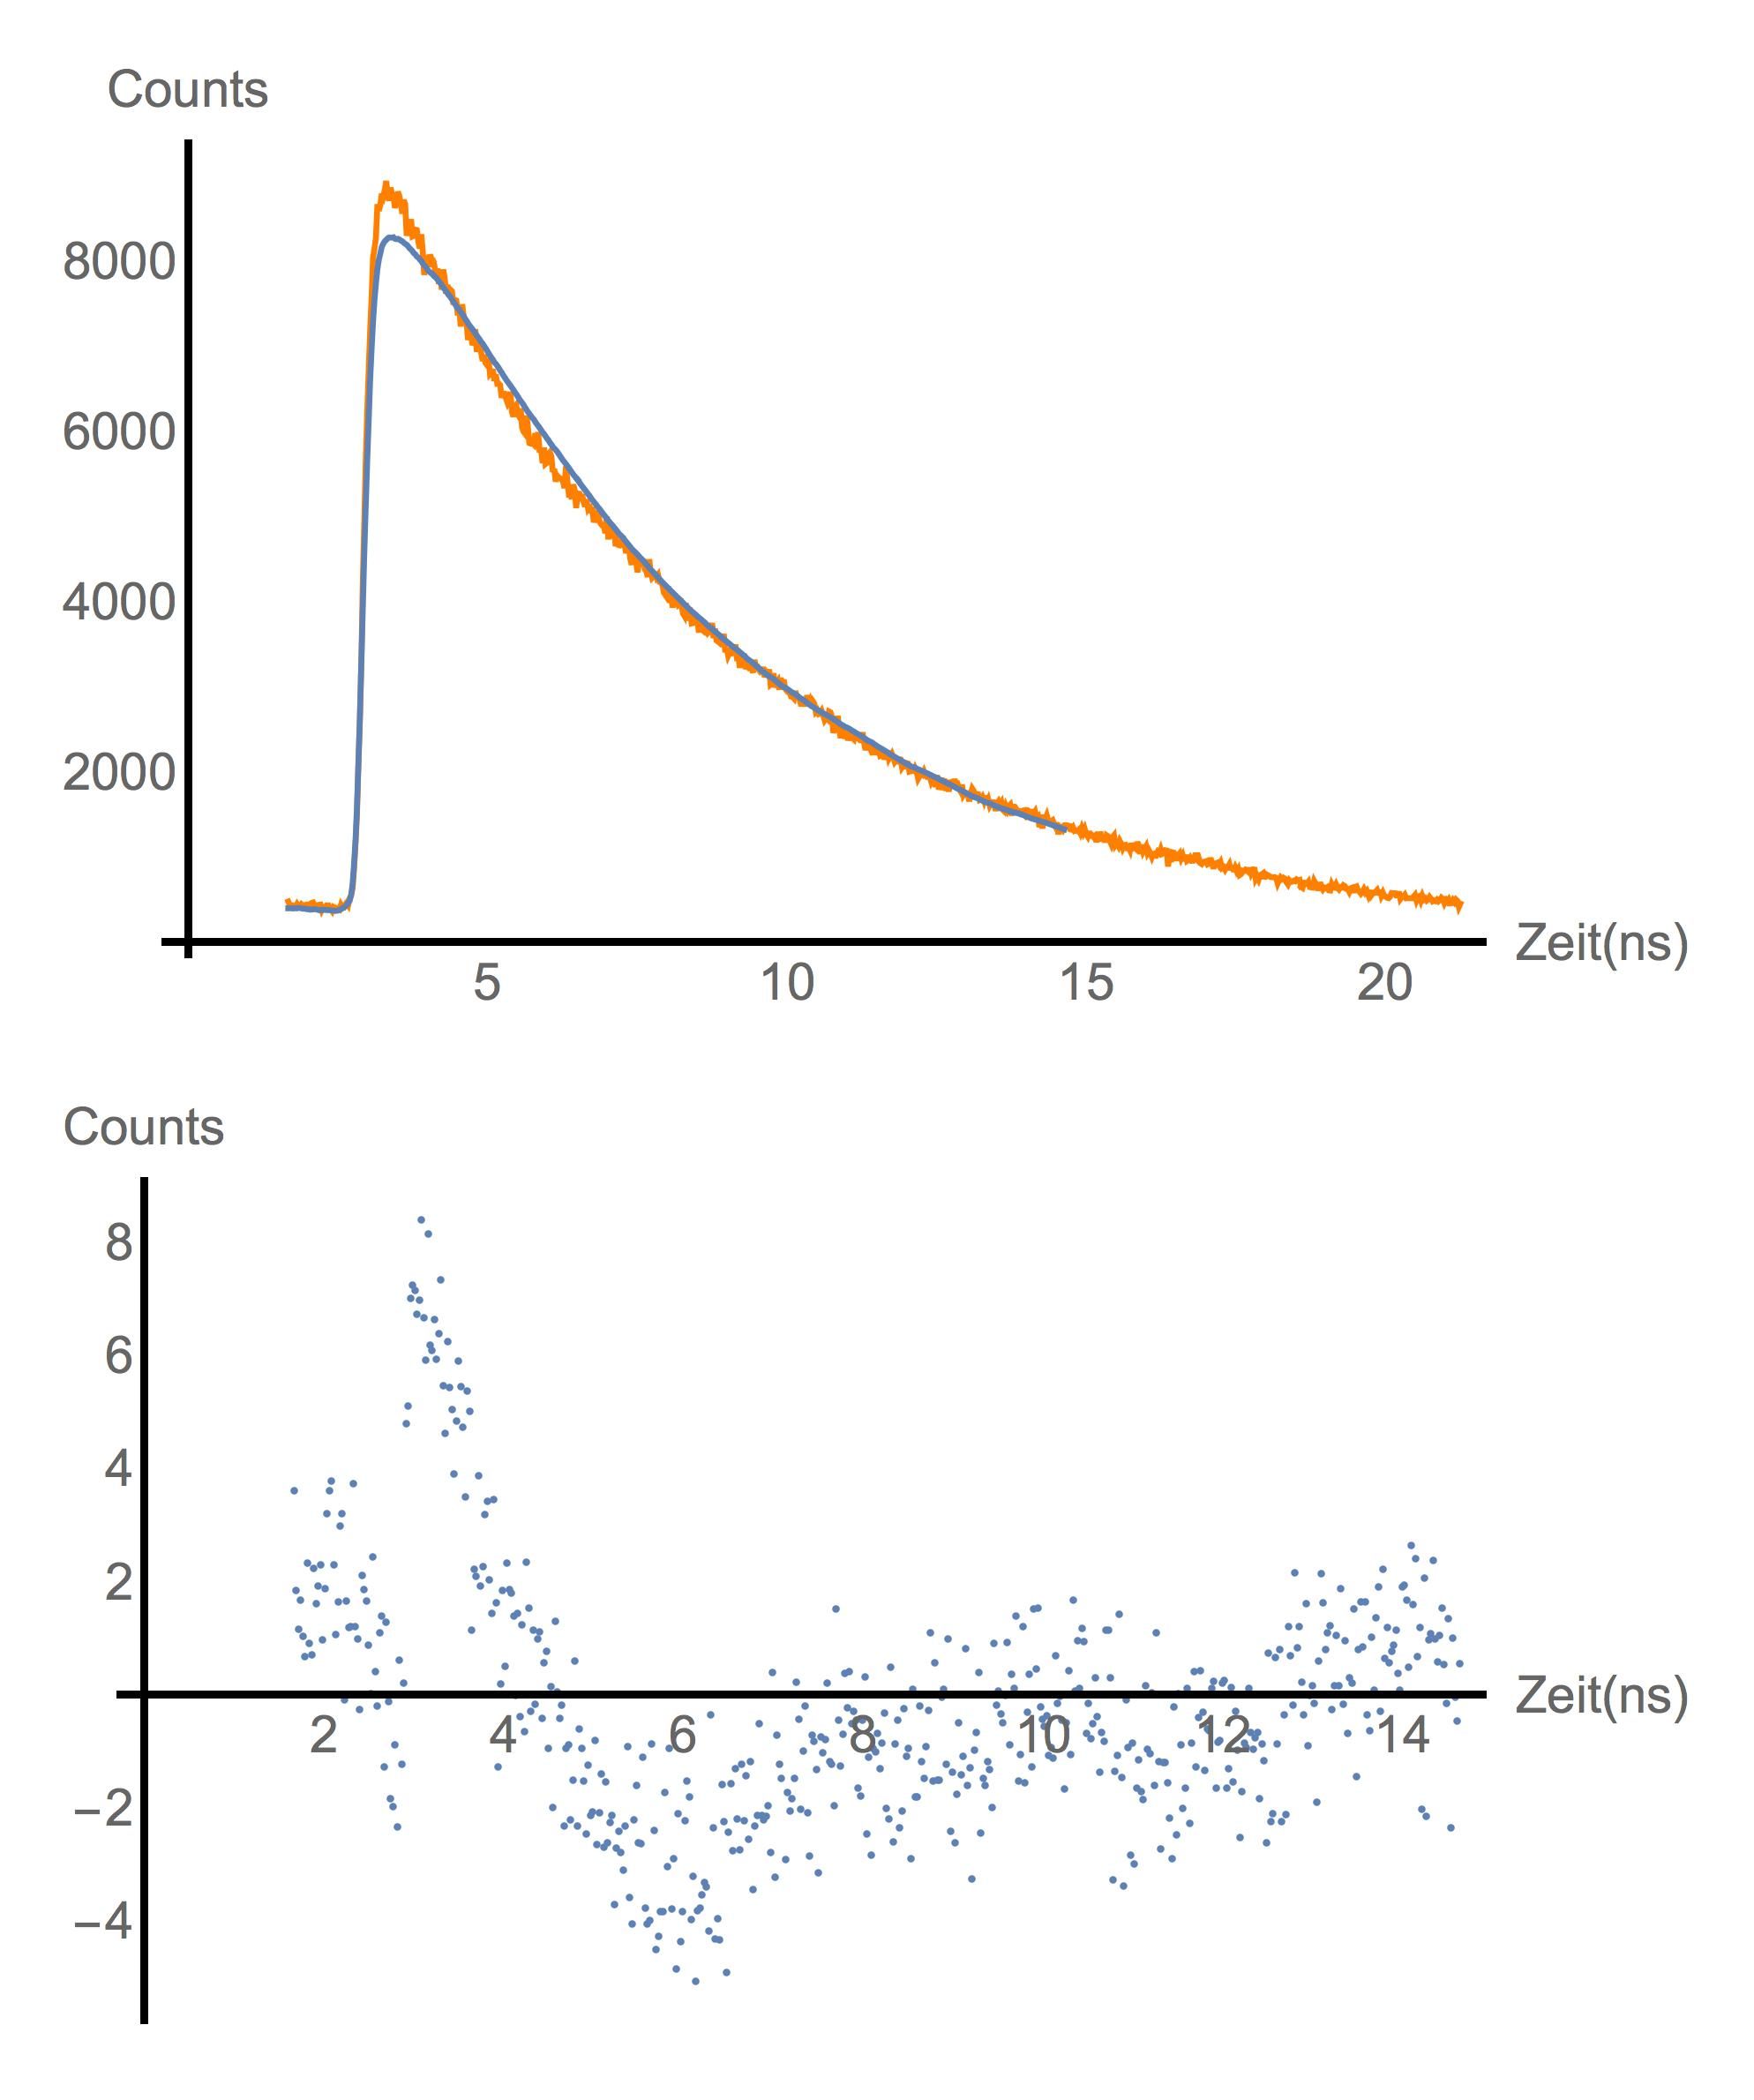
\includegraphics[width=\textwidth/2]{Bilder/Fit9100uW.jpg}\\
  (c) I = 79 $\mu$W, $\chi^2$=2.06                               &   (d) I = 91 $\mu$W, $\chi^2$=2.44                             \\

\end{tabular}
\caption{Fits und Residuen des Peak-Pile-Up-Effekts}
\end{figure}


\begin{figure}
  \centering
  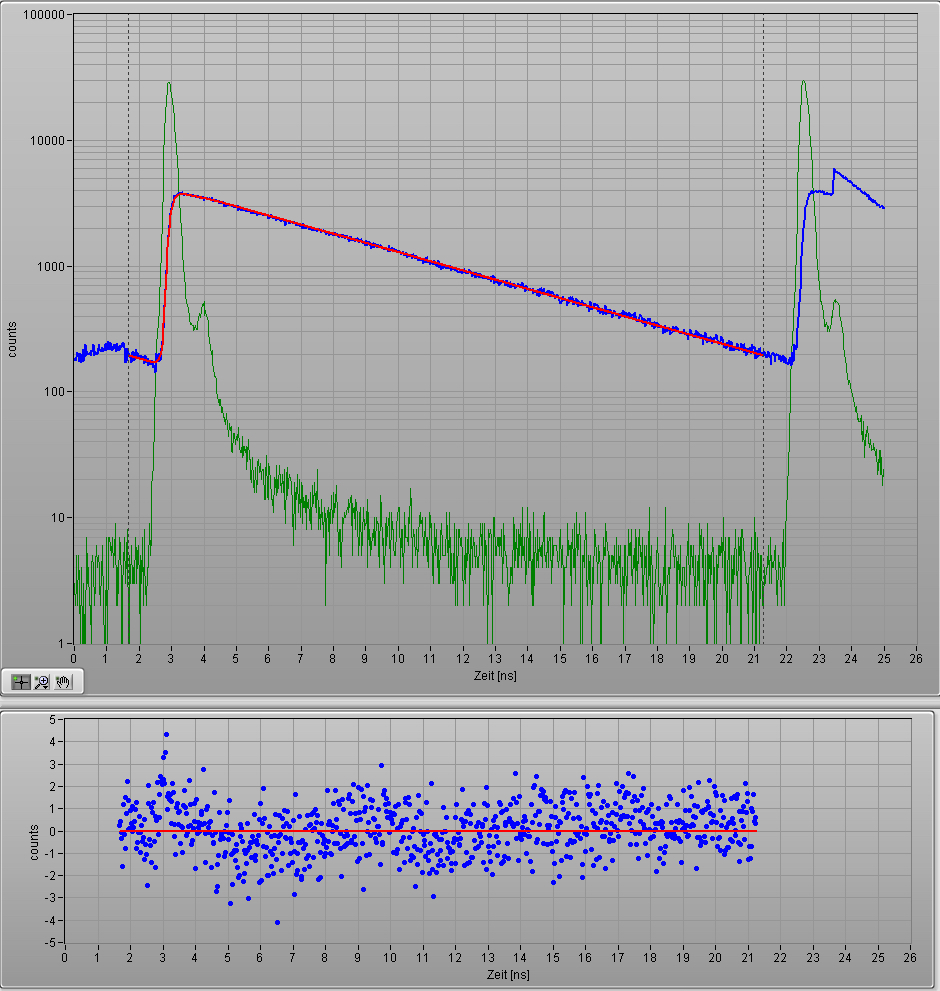
\includegraphics[width=\textwidth]{Bilder/messung_opt.jpg}
  \caption{Mess- und Fitkurve für optimale Einstellung, Fitparameter: $t=5.91ns$, $A=0.001[a.u.]$, $\chi^2=1.24$}
\end{figure}


\newpage


\section{Literatur}

\begingroup
\renewcommand{\section}[2]{}
\begin{thebibliography}{20}
        \bibitem{Hackbarth} Dr. Steffen Hackbarth: \textit{Versuchsskript: Zeitkorrelierte Einzelphotonenmessung}
        \bibitem{Roeder} Röder et al.: \textit{Photophysical properties of pheophorbide a in solution and in model membrane systems}
\end{thebibliography}
\endgroup

\end{document}
